% 若编译失败,且生成 .synctex(busy) 辅助文件,可能有两个原因:
% 1. 需要插入的图片不存在:Ctrl + F 搜索 'figure' 将这些代码注释/删除掉即可
% 2. 路径/文件名含中文或空格:更改路径/文件名即可

% ------------------------------------------------------------- %
% >> ------------------ 文章宏包及相关设置 ------------------ << %
% 设定文章类型与编码格式
    \documentclass[UTF8]{report}		

% 本 .tex 专属的宏定义
    \def\V{\ \mathrm{V}}
    \def\mV{\ \mathrm{mV}}
    \def\kV{\ \mathrm{KV}}
    \def\KV{\ \mathrm{KV}}
    \def\MV{\ \mathrm{MV}}
    \def\A{\ \mathrm{A}}
    \def\mA{\ \mathrm{mA}}
    \def\kA{\ \mathrm{KA}}
    \def\KA{\ \mathrm{KA}}
    \def\MA{\ \mathrm{MA}}
    \def\O{\ \Omega}
    \def\mO{\ \Omega}
    \def\kO{\ \mathrm{K}\Omega}
    \def\KO{\ \mathrm{K}\Omega}
    \def\MO{\ \mathrm{M}\Omega}
    \def\Hz{\ \mathrm{Hz}}

% 自定义宏定义
    \def\N{\mathbb{N}}
    \def\F{\mathbb{F}}
    \def\Z{\mathbb{Z}}
    \def\Q{\mathbb{Q}}
    \def\R{\mathbb{R}}
    \def\C{\mathbb{C}}
    \def\T{\mathbb{T}}
    \def\S{\mathbb{S}}
    \def\A{\mathbb{A}}
    \def\I{\mathscr{I}}
    \def\Im{\mathrm{Im\,}}
    \def\Re{\mathrm{Re\,}}
    \def\d{\mathrm{d}}
    \def\p{\partial}
% 导入基本宏包
    \usepackage[UTF8]{ctex}     % 设置文档为中文语言
    \usepackage[colorlinks, linkcolor=blue, anchorcolor=blue, citecolor=blue, urlcolor=blue]{hyperref}  % 宏包:自动生成超链接 (此宏包与标题中的数学环境冲突)
    % \usepackage{docmute}    % 宏包:子文件导入时自动去除导言区,用于主/子文件的写作方式,\include{./51单片机笔记}即可。注:启用此宏包会导致.tex文件capacity受限。
    \usepackage{amsmath}    % 宏包:数学公式
    \usepackage{mathrsfs}   % 宏包:提供更多数学符号
    \usepackage{amssymb}    % 宏包:提供更多数学符号
    \usepackage{pifont}     % 宏包:提供了特殊符号和字体
    \usepackage{extarrows}  % 宏包:更多箭头符号


% 文章页面margin设置
    \usepackage[a4paper]{geometry}
        \geometry{top=1in}
        \geometry{bottom=1in}
        \geometry{left=0.75in}
        \geometry{right=0.75in}   % 设置上下左右页边距
        \geometry{marginparwidth=1.75cm}    % 设置边注距离(注释、标记等)

% 配置数学环境
    \usepackage{amsthm} % 宏包:数学环境配置
    % theorem-line 环境自定义
        \newtheoremstyle{MyLineTheoremStyle}% <name>
            {11pt}% <space above>
            {11pt}% <space below>
            {}% <body font> 使用默认正文字体
            {}% <indent amount>
            {\bfseries}% <theorem head font> 设置标题项为加粗
            {:}% <punctuation after theorem head>
            {.5em}% <space after theorem head>
            {\textbf{#1}\thmnumber{#2}\ \ (\,\textbf{#3}\,)}% 设置标题内容顺序
        \theoremstyle{MyLineTheoremStyle} % 应用自定义的定理样式
        \newtheorem{LineTheorem}{Theorem.\,}
    % theorem-block 环境自定义
        \newtheoremstyle{MyBlockTheoremStyle}% <name>
            {11pt}% <space above>
            {11pt}% <space below>
            {}% <body font> 使用默认正文字体
            {}% <indent amount>
            {\bfseries}% <theorem head font> 设置标题项为加粗
            {:\\ \indent}% <punctuation after theorem head>
            {.5em}% <space after theorem head>
            {\textbf{#1}\thmnumber{#2}\ \ (\,\textbf{#3}\,)}% 设置标题内容顺序
        \theoremstyle{MyBlockTheoremStyle} % 应用自定义的定理样式
        \newtheorem{BlockTheorem}[LineTheorem]{Theorem.\,} % 使用 LineTheorem 的计数器
    % definition 环境自定义
        \newtheoremstyle{MySubsubsectionStyle}% <name>
            {11pt}% <space above>
            {11pt}% <space below>
            {}% <body font> 使用默认正文字体
            {}% <indent amount>
            {\bfseries}% <theorem head font> 设置标题项为加粗
            {:\\ \indent}% <punctuation after theorem head>
            {0pt}% <space after theorem head>
            {\textbf{#3}}% 设置标题内容顺序
        \theoremstyle{MySubsubsectionStyle} % 应用自定义的定理样式
        \newtheorem{definition}{}

%宏包:有色文本框(proof环境)及其设置
    \usepackage[dvipsnames,svgnames]{xcolor}    %设置插入的文本框颜色
    \usepackage[strict]{changepage}     % 提供一个 adjustwidth 环境
    \usepackage{framed}     % 实现方框效果
        \definecolor{graybox_color}{rgb}{0.95,0.95,0.96} % 文本框颜色。修改此行中的 rgb 数值即可改变方框纹颜色,具体颜色的rgb数值可以在网站https://colordrop.io/ 中获得。(截止目前的尝试还没有成功过,感觉单位不一样)(找到喜欢的颜色,点击下方的小眼睛,找到rgb值,复制修改即可)
        \newenvironment{graybox}{%
        \def\FrameCommand{%
        \hspace{1pt}%
        {\color{gray}\small \vrule width 2pt}%
        {\color{graybox_color}\vrule width 4pt}%
        \colorbox{graybox_color}%
        }%
        \MakeFramed{\advance\hsize-\width\FrameRestore}%
        \noindent\hspace{-4.55pt}% disable indenting first paragraph
        \begin{adjustwidth}{}{7pt}%
        \vspace{2pt}\vspace{2pt}%
        }
        {%
        \vspace{2pt}\end{adjustwidth}\endMakeFramed%
        }

% 外源代码插入设置
    % matlab 代码插入设置
    \usepackage{matlab-prettifier}
        \lstset{
            style=Matlab-editor,  % 继承matlab代码颜色等
        }
    \usepackage[most]{tcolorbox} % 引入tcolorbox包 
    \usepackage{listings} % 引入listings包
        \tcbuselibrary{listings, skins, breakable}
        \newfontfamily\codefont{Consolas} % 定义需要的 codefont 字体
        \lstdefinestyle{matlabstyle}{
            language=Matlab,
            basicstyle=\small\ttfamily\codefont,    % ttfamily 确保等宽 
            breakatwhitespace=false,
            breaklines=true,
            captionpos=b,
            keepspaces=true,
            numbers=left,
            numbersep=15pt,
            showspaces=false,
            showstringspaces=false,
            showtabs=false,
            tabsize=2
        }
        \newtcblisting{matlablisting}{
            arc=2pt,        % 圆角半径
            top=-5pt,
            bottom=-5pt,
            left=1mm,
            listing only,
            listing style=matlabstyle,
            breakable,
            colback=white   % 选一个合适的颜色
        }

% table 支持
    \usepackage{booktabs}   % 宏包:三线表
    \usepackage{tabularray} % 宏包:表格排版
    \usepackage{longtable}  % 宏包:长表格
    \usepackage[longtable]{multirow} % 宏包:multi 行列

% figure 设置
    \usepackage{graphicx}   % 支持 jpg, png, eps, pdf 图片 
    \usepackage{svg}        % 支持 svg 图片
    \usepackage{subcaption} % 支持子图
        \svgsetup{
            % 指向 inkscape.exe 的路径
            inkscapeexe = D:/aa_my_apps_main/Inkscape/bin/inkscape.exe, 
            % 一定程度上修复导入后图片文字溢出几何图形的问题
            inkscapelatex = false                 
        }

% 图表进阶设置
    \usepackage{caption}    % 图注、表注
        \captionsetup[figure]{name=图}  
        \captionsetup[table]{name=表}
        \captionsetup{labelfont=bf, font=small}
    \usepackage{float}     % 图表位置浮动设置 

% 圆圈序号自定义
    \newcommand*\circled[1]{\tikz[baseline=(char.base)]{\node[shape=circle,draw,inner sep=0.8pt, line width = 0.03em] (char) {\small \bfseries #1};}}   % TikZ solution

% 列表设置
    \usepackage{enumitem}   % 宏包:列表环境设置
        \setlist[enumerate]{
            label=\bfseries(\arabic*) ,   % 设置序号样式为加粗的 (1) (2) (3)
            ref=\arabic*, % 如果需要引用列表项,这将决定引用格式(这里仍然使用数字)
            itemsep=0pt, parsep=0pt, topsep=0pt, partopsep=0pt, leftmargin=3.5em} 
        \setlist[itemize]{itemsep=0pt, parsep=0pt, topsep=0pt, partopsep=0pt, leftmargin=3.5em}
        \newlist{circledenum}{enumerate}{1} % 创建一个新的枚举环境  
        \setlist[circledenum,1]{  
            label=\protect\circled{\arabic*}, % 使用 \arabic* 来获取当前枚举计数器的值,并用 \circled 包装它  
            ref=\arabic*, % 如果需要引用列表项,这将决定引用格式(这里仍然使用数字)
            itemsep=0pt, parsep=0pt, topsep=0pt, partopsep=0pt, leftmargin=3.5em
        }  
    

% 文章默认字体设置
    \usepackage{fontspec}   % 宏包:字体设置
        \setmainfont{SimSun}    % 设置中文字体为宋体字体
        \setmainfont{Times New Roman} % 设置英文字体为Times New Roman

% 其它设置
    % 脚注设置
    \renewcommand\thefootnote{\ding{\numexpr171+\value{footnote}}}
    % 参考文献引用设置
        \bibliographystyle{unsrt}   % 设置参考文献引用格式为unsrt
        \newcommand{\upcite}[1]{\textsuperscript{\cite{#1}}}     % 自定义上角标式引用
    % 文章序言设置
        \newcommand{\cnabstractname}{序言}
        \newenvironment{cnabstract}{%
            \par\Large
            \noindent\mbox{}\hfill{\bfseries \cnabstractname}\hfill\mbox{}\par
            \vskip 2.5ex
            }{\par\vskip 2.5ex}
% 各级标题自定义设置
    \usepackage{titlesec}   
    % chapter
        \titleformat{\chapter}[hang]{\normalfont\Large\bfseries\centering}{Homework \thechapter :}{10pt}{}
        \titlespacing*{\chapter}{0pt}{-30pt}{10pt} % 控制上方空白的大小
    % section
        \titleformat{\section}[hang]{\normalfont\large\bfseries}{\thesection}{8pt}{}
    % subsection
        %\titleformat{\subsubsection}[hang]{\normalfont\bfseries}{}{8pt}{}
    % subsubsection
        %\titleformat{\subsubsection}[hang]{\normalfont\bfseries}{}{8pt}{}

% >> ------------------ 文章宏包及相关设置 ------------------ << %
% ------------------------------------------------------------- %



% ----------------------------------------------------------- %
% >> --------------------- 文章信息区 --------------------- << %
% 页眉页脚设置

\usepackage{fancyhdr}   %宏包:页眉页脚设置
    \pagestyle{fancy}
    \fancyhf{}
    \cfoot{\thepage}
    \renewcommand\headrulewidth{1pt}
    \renewcommand\footrulewidth{0pt}
    \chead{某某课程作业模版,\ 丁毅,\ 2023K8009908031}
    \lhead{Homework \thechapter}
    \rhead{dingyi233@mails.ucas.ac.cn}

%文档信息设置
\title{某某课程作业模版\\ Template of Homework}
\author{丁毅\\ \footnotesize 中国科学院大学,北京 100049\\ Yi Ding \\ \footnotesize University of Chinese Academy of Sciences, Beijing 100049, China}
\date{\footnotesize 2024.8 -- 2025.1}
% >> --------------------- 文章信息区 --------------------- << %
% ----------------------------------------------------------- %

% 开始编辑文章

\begin{document}
\zihao{5}           % 设置全文字号大小

% --------------------------------------------------------------- %
% >> --------------------- 封面序言与目录 --------------------- << %
% 封面
    \maketitle\newpage  
    \pagenumbering{Roman} % 页码为大写罗马数字
    \thispagestyle{fancy}   % 显示页码、页眉等

% 序言
    \begin{cnabstract}\normalsize 
        本文为笔者本科时的“电路原理”课程作业(Homework of Circuit Theory, 2024.9-2025.1)。由于个人学识浅陋,认识有限,文中难免有不妥甚至错误之处,望读者不吝指正,在此感谢。\par 
        我的邮箱是 dingyi233@mails.ucas.ac.cn。
    \end{cnabstract}
    \addcontentsline{toc}{chapter}{序言} % 手动添加为目录

% 不换页目录
    \setcounter{tocdepth}{0}
    \noindent\rule{\textwidth}{0.1em}   % 分割线
    \noindent\begin{minipage}{\textwidth}\centering 
        \vspace{1cm}
        \tableofcontents\thispagestyle{fancy}   % 显示页码、页眉等   
    \end{minipage}  
    \addcontentsline{toc}{chapter}{目录} % 手动添加为目录

% 收尾工作
    \newpage    
    \pagenumbering{arabic} 

% >> --------------------- 封面序言与目录 --------------------- << %
% --------------------------------------------------------------- %


\chapter{2024.8.27 - 2024.9.2}\thispagestyle{fancy}

\section{习题集 1-2}

\begin{enumerate}
\item[(a)] 短路,因此 $U = 0,\  I = \frac{U_S}{R_i}$
\item[(b)] 开路,因此 $U = U_s, \ I = 0$
\item[(c)] 构成回路,因此  $ U = \frac{U_SR}{R + R_i},\ I = \frac{U_S}{R + R_i}$ 
\end{enumerate}

\begin{figure}[H]\centering
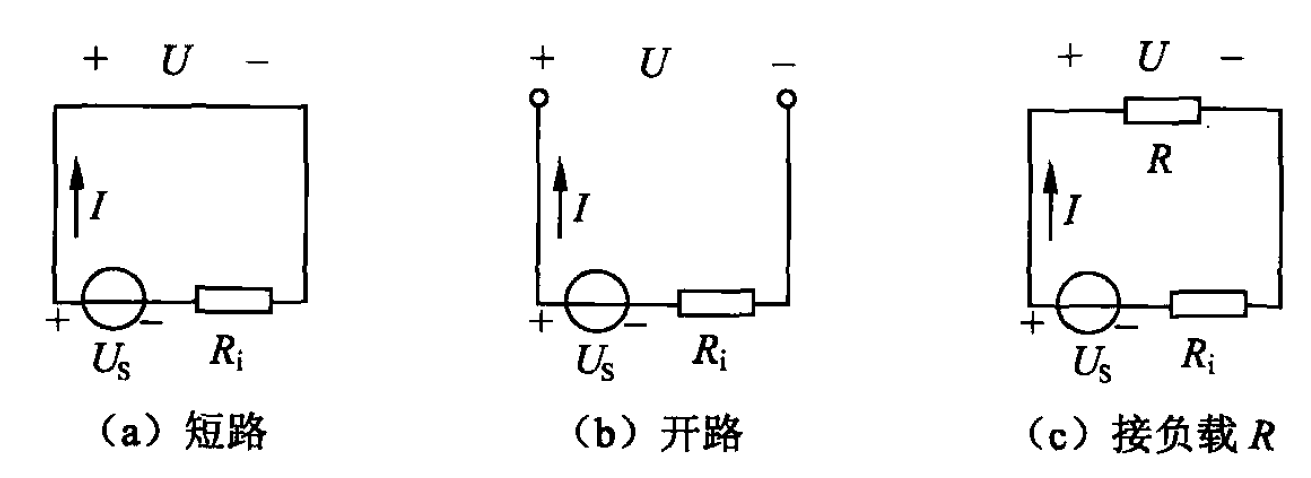
\includegraphics[width=0.6\textwidth]{assets/1/ae1cfc03fad5c98bfff08a663714a004.png}
\end{figure}

\section{习题集 1-9}

\begin{enumerate}
    \item[(a)]  $ \varphi_a - 3\ \mathrm{V} + 2\ \mathrm{V} = \varphi_b \Longrightarrow U_{ab} = 1\ \mathrm{V} $ 
    \item[(b)] $I = 1\ \mathrm{A},\  3 -IR= -4 \Longrightarrow R = 7\ \Omega$ 
    \item[(c)] $-3 + U_S = 1 \Longrightarrow U_S = 4 \ \mathrm{V}$ 
    \item[(d)] $R=2\ \Omega,\ -IR + 2 = 3 \Longrightarrow I = -0.5\ \mathrm{A}$ 
\end{enumerate}

\begin{figure}[H]\centering
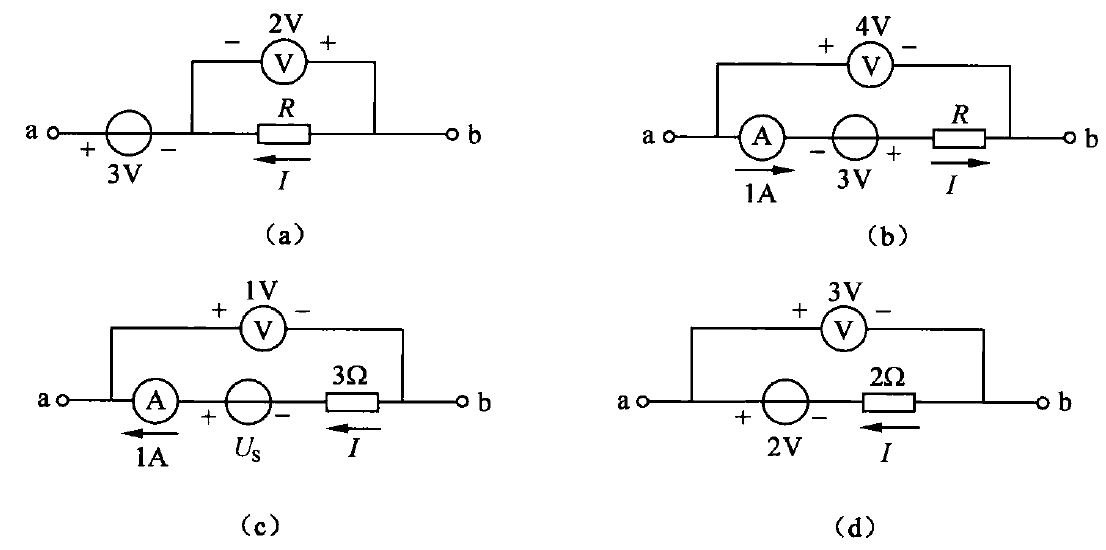
\includegraphics[width=0.6\textwidth]{assets/1/d3d69ecd6b1c1bc476fd4a4957fb9e56.png}
\end{figure}

\section{习题集 1-10}



\begin{enumerate}
\item[(a)] 
记参考点 a 的电势 $\varphi_a=0$,则 $\varphi_c = 2\ \mathrm{V} ,\ \varphi_b = -2\ \mathrm{V}$,因此 $U_{ab} = 2\ \mathrm{V}$

\item[(b)] 
记参考点 d 的电势 $\varphi_d = \varphi_b =0$,则 $\varphi_c = 6\ \mathrm{V},\ \varphi_a = -2\ \mathrm{V}$,因此 $U_{ab} = -2\ \mathrm{V}$

\end{enumerate}

\begin{figure}[H]\centering
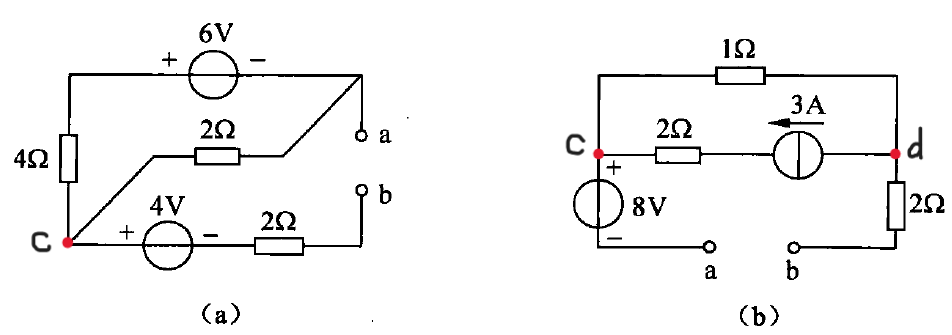
\includegraphics[width=0.55\textwidth]{assets/1/9dda9e5f333b8cb7f498d15c015e5fd0.png}
\end{figure}
{\par\color{gray}\small
后补:(b) 中电流源两端仍有电势差,$\varphi_c \ne 6 \ \mathrm{V}$ 而是 $ \varphi_c = -3\ \mathrm{V} $,最终得 $U_{ab} = -5 \ \mathrm{V}$。
\par}


\section{习题集 1-15}

\begin{enumerate}
    \item[(a)] $I = -\frac{U}{R} + 4\ \mathrm{A} = -2 \ \mathrm{A}$
    \item[(b)] $U =12 \ \mathrm{V} + 3\ \Omega \times 4 \ \mathrm{A} = 0 $ 
    \item[(c)] $I = 8 \ \mathrm{A} - 6\ \mathrm{A} = 2 \ \mathrm{A}$,$ U = 12 \ \mathrm{V} + 3\times8 \ \mathrm{V} = 36 \ \mathrm{V}$ 
    \item[(d)] 取点 $ d $ 为参考点,则 $\varphi_d = \varphi_c = 0$,$\varphi_b = \varphi_a = 9 \ \mathrm{V}$,于是 $U_1 = 9 + 2\times3 = 15\ \mathrm{V},\ U_2 = 9 + 2\times 2 = 13 \ \mathrm{V},\ I =2 -  (9-3) = - 4 \ \mathrm{A}$
\end{enumerate}

\begin{figure}[H]\centering
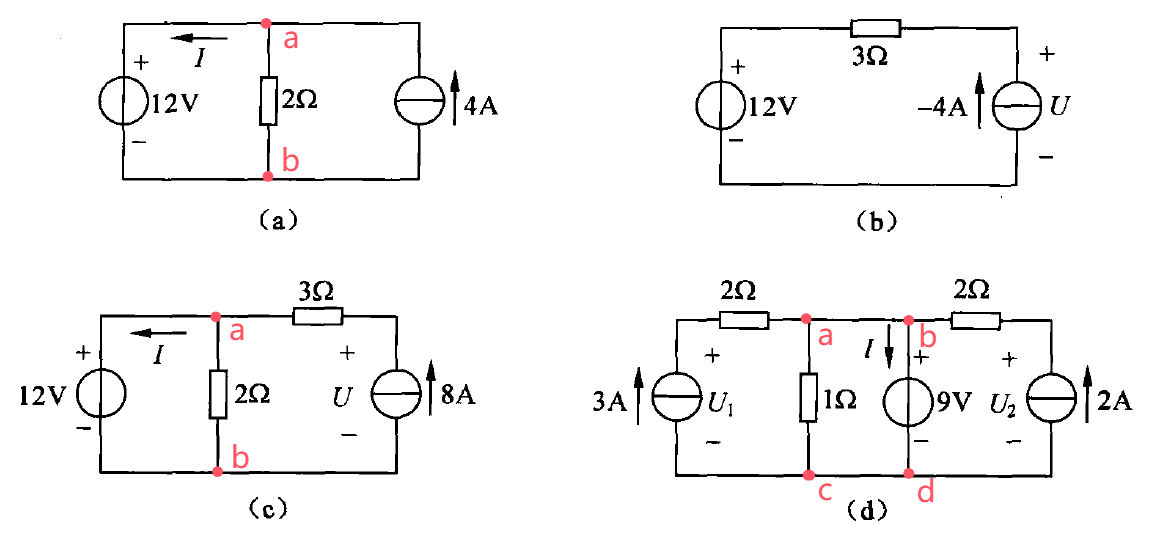
\includegraphics[width=0.7\textwidth]{assets/1/b82ef4f3b4efd9d0ee903e5f19353345.png}
\end{figure}

\section{习题集 1-29}

取点 $a$ 为参考点 $\varphi_a = 0$,可得 $\varphi_b = 100U_1 - 80$,于是在结点 $a$ 有电流:
\begin{equation*}
I_S + \frac{100U_1 - 80}{5} = 2
\end{equation*}

$0.2\ \Omega$ 电阻处又有 $U_1 = 0.2 I_S$,联立解得 $I_S = 3.6 \ \mathrm{A}, U_1 = 7.2 \ \mathrm{V}$。

\section{习题集 1-30}

这里要注意左二元器件是受控电流源,因此 $0.5U$ 是指电流大小而非电压。$I_1$ 处可列出方程:

\begin{equation*}
\frac{U}{2} + 12 - \frac{U}{3} = 0.5U \Longrightarrow U = 36 \ \mathrm{V} \Longrightarrow P = UI = 432 \ \mathrm{W}
\end{equation*}

\begin{figure}[H]\centering
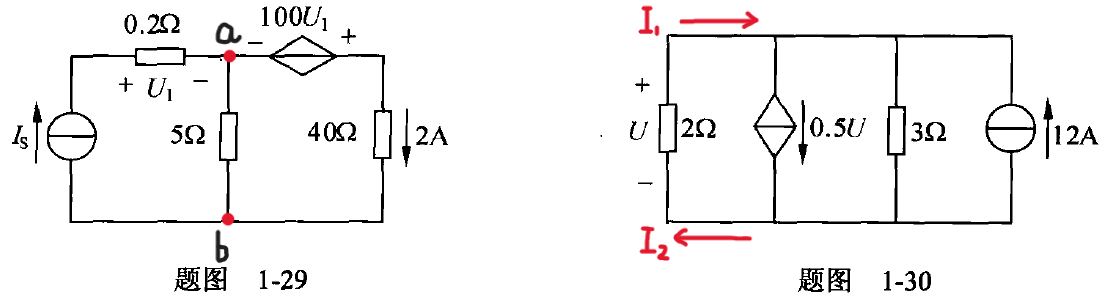
\includegraphics[width=0.7\textwidth]{assets/1/94b342032a5f6622a60b3c9d99e37993.png}
\end{figure}

{\par\color{gray}\small
后补:上面的方程列错了,错将 $I_1$ 的方向标为由左向右,应该是由右向左。最后得到 $P = 108\ \mathrm{W}$。另外,也可以直接将受控电流源看作是 2 $\Omega$ 的电阻,这样左侧三个电阻并联,也可求出正确答案 108 W.
\par}


\section{讲义题 1-6}

$\alpha > 90 \text{\textdegree}$ 时,电阻为“负电阻”。

\section{讲义题 1-7}


\begin{definition}[充放电倍率 C 的含义]
C (充放电倍率)表示电池充放电时电流相对电池容量的大小数值,$\mathrm{C} = \frac{\text{电池容量}}{\text{充放电所需时间}}$。例如,1 C 电流充电表示电池需要 1 小时充满,5 C 充电表示电池需要 $0.2$ 小时充满。放电也是类似的,一个 10 Ah 的电池以 2 C 放电,表示以 20 A 的电流放电 0.5 h。 \par
若倍率上升,总时间就会下降,若倍率下降,总时间就会上升。通俗来讲,$C$ 代表了电池的爆发力大小,高倍率的动力电池瞬间放电电流大,特别适合大电流放电产品使用,如航模。
\end{definition}


\begin{definition}[涓流充电]
涓流充电是指在电池接近完全充满电后,采用非常小的电流进行充电,以弥补电池自放电造成的容量损失。理论倍率 C 约为 最大倍率 $\mathrm{C_{max}}$ 的 $\frac{1}{100}$ 至 $\frac{1}{1000}$,但由于倍率太小,常常根本无法充电,一个比较好的方法是脉冲式充电,例如以 $\frac{\mathrm{C_{max}}}{10}$ 充电 6 s,然后停止充电 54 s。
\end{definition}


\begin{definition}[快速充电]
快速充电至少要求 1 C,现阶段的快速充电多在 1.5 C 至 2 C 之间。
\end{definition}


\section{讲义题 1-8(Multisim 仿真)}

仿真电路如图 \ref{仿真电路图} 所示,

\begin{figure}[H]\centering
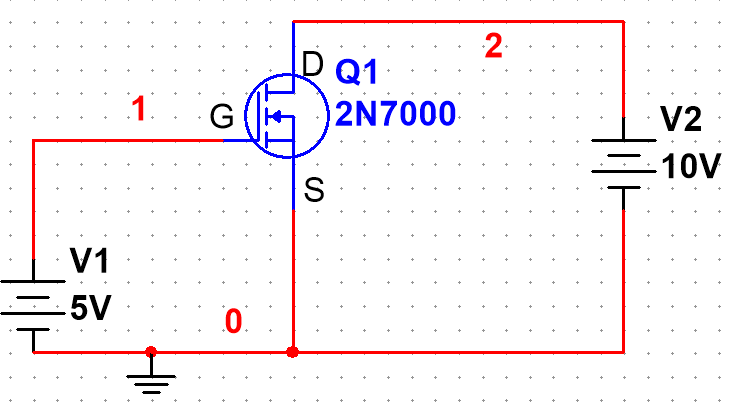
\includegraphics[width=0.36\textwidth]{assets/1/5c45ed5b5258df3fa8e1babac4a7ace2.png}
\caption{\textbf{仿真电路图}}\label{仿真电路图}
\end{figure}

先固定 $U_{GS} = 5\ \mathrm{V}$ 不变(即 $V_1 = 5\ \mathrm{V}$),横坐标 $U_{DS} \in [0\ \mathrm{V},\ 12\ \mathrm{V}]$,画出 $I_{DS}$(即 $I_2$)的变化曲线,如图 \ref{仿真结果1} 所示。再固定 $U_{DS} = 10\ \mathrm{V}$ 不变(即 $V_2 = 10\ \mathrm{V}$),横坐标 $U_{GS} \in [0\ \mathrm{V},\ 10\ \mathrm{V}]$,画出 $I_{DS}$(即 $I_2$)的变化曲线,如图 \ref{仿真结果2} 所示。
\begin{center}
    \noindent\begin{minipage}{0.42\textwidth}
        \begin{figure}[H]\centering
        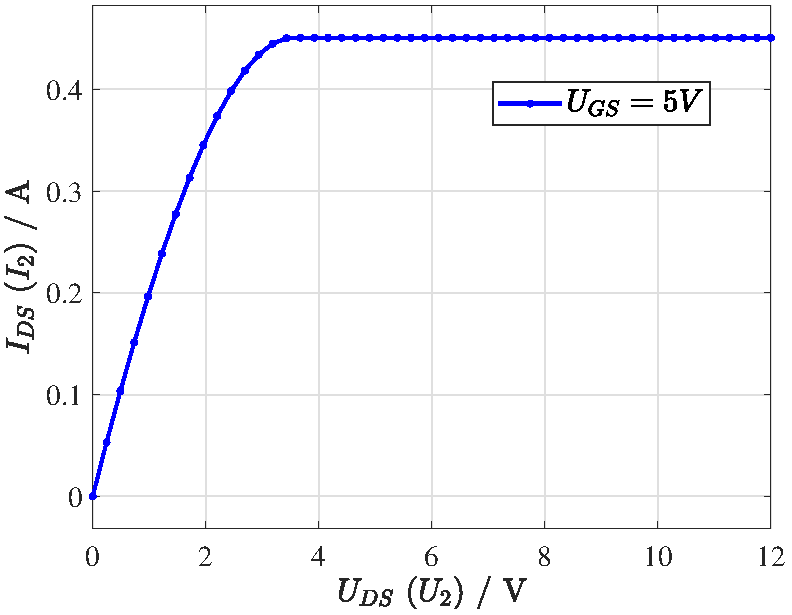
\includegraphics[width=\textwidth]{assets/1/2024-08-30_00-57-32.pdf}
        \caption{\textbf{仿真结果1}}\label{仿真结果1}
        \end{figure}
    \end{minipage}\hspace{5mm}
    \begin{minipage}{0.42\textwidth}
        \begin{figure}[H]\centering
        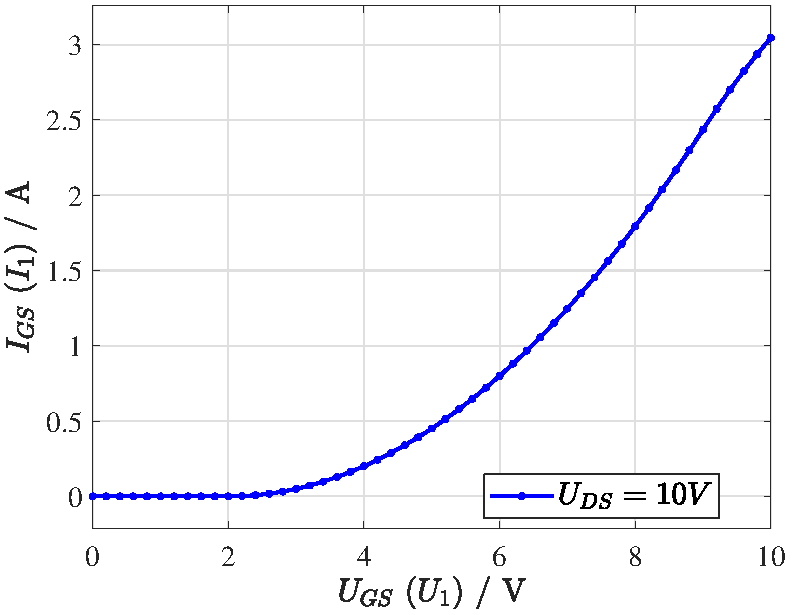
\includegraphics[width=\textwidth]{assets/1/2024-08-30_00-57-34.pdf}
    \caption{\textbf{仿真结果2}}\label{仿真结果2}
    \end{figure}
    \end{minipage}
\end{center}


\chapter{2024.9.10 - 2024.9.19}\thispagestyle{fancy}


\section{习题集 3-40(书上答案不正确)}

由虚短和虚断,可以得到 $R_1$ 处电流为 $i_1 = \frac{u_s}{R_1}$(从上至下),于是输出电压 $u_o = 3u_s$,右侧负载由三个电阻构成,并联电阻分压 $2u_s$,最后得电流 $i(t)$:
\begin{equation}
i(t) = \frac{2u_s}{6 \KO} = \frac{u_s}{3} \mA
\end{equation}

\begin{figure}[H]\centering
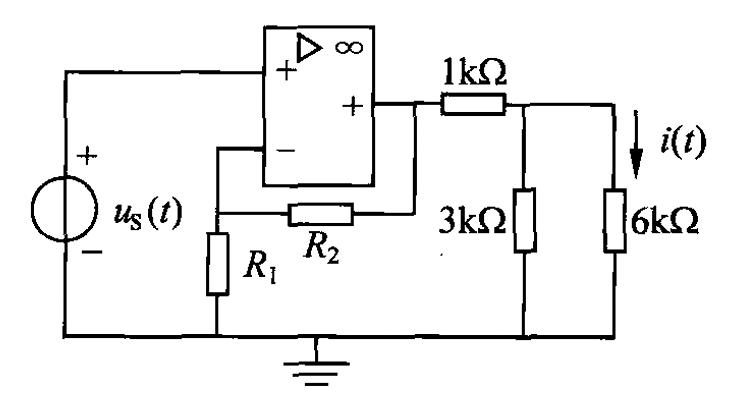
\includegraphics[width=0.4\textwidth]{assets/3/3-40.jpg}
\caption{\bfseries 习题集 3-40}
\end{figure}

\section{习题集 3-45(注意题目单位是 S)}

如图所示,将电导全部转换为电阻。由虚断、虚短,流经 $\frac{1}{10}\ \Omega$ 电阻的电流为 $i_1 = \frac{u_s}{0.1\ \Omega} = 10u_s$。右下角两电阻分压,再由虚短可得 $i_2 = 2U_o$,于是 $i_3 = i_1 + i_2 = 10 U_s + 2U_o$,由 KVL:
\begin{equation}
0 - \frac{1}{3}(10 U_s + 2U_o) = U_o \Longrightarrow  \frac{U_o}{U_s} = -2
\end{equation}
入端电阻 $R_i$: 
\begin{equation}
    i_1 = 10U_s \Longrightarrow  R_i = \frac{1}{10}\ \Omega
\end{equation}

\section{习题集 3-46}

依据 KVL、KCL、虚短、虚断,标出各节点电势,如图所示。则有:
\begin{equation}
(u_i+u_o)-u_o = i_LR,\ i_L = \frac{u_o}{R_L} \Longrightarrow u_o = u_i,\ i_L = \frac{u_o}{R_L} = \frac{u_i}{R_L}
\end{equation}

\begin{figure}[H]\centering
    \begin{subfigure}[t]{0.43\textwidth}\centering
        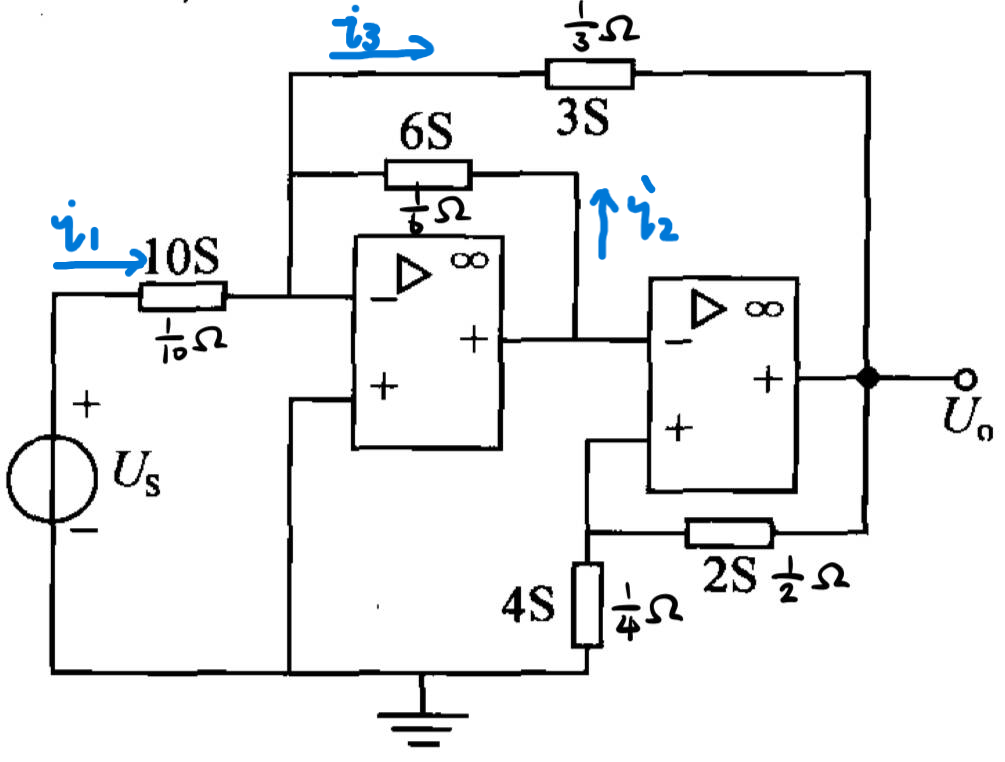
\includegraphics[height=150pt]{assets/3/3-45.png}
        \caption{\bfseries 习题集 3-45 }
    \end{subfigure}\begin{subfigure}[t]{0.43\textwidth}\centering
        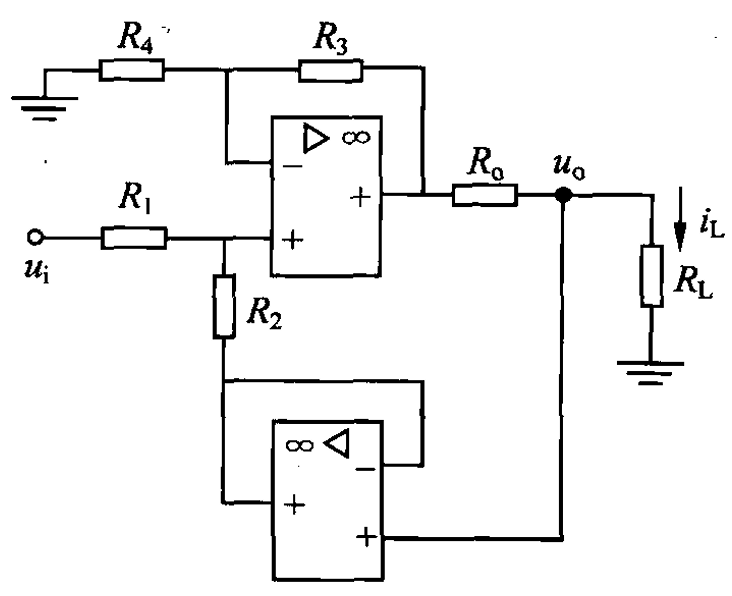
\includegraphics[height=150pt]{assets/3/3-46.png}
        \caption{\bfseries 习题集 3-46 }
    \end{subfigure}
    \caption{\bfseries 习题集 3-45 和习题集 3-46 }
    \end{figure}
    


\section{讲义题 2-19}
\textbf{(1)\ 反相比例放大器}

对输入电阻,$i_1 = \frac{u_i}{R_1} \Longrightarrow R_i = R_1$。对输出电阻,将输入电压源短路,采用加流求压法,在输出端接入电流源,由 $u = iR$ 且 $u=0$,得 $R_o = 0$。也即:
\begin{equation}
R_i = R_1,\ R_o = 0
\end{equation}

\textbf{(2)\ 同相比例放大器}

对输入电阻,$R_1$ 右端断路,因此 $R_i = \infty$。对输出电阻,将输入电压源短路,采用加流求压法,在输出端接入电流源,由 $u = iR$ 且 $u=0$,得 $R_o = 0$。也即:
\begin{equation}
R_i = \infty,\ R_o = 0
\end{equation}

从输入输出电阻特性来看,同相比例放大器电气特性更优秀。

\begin{figure}[H]\centering
\begin{subfigure}[t]{0.4\textwidth}\centering
    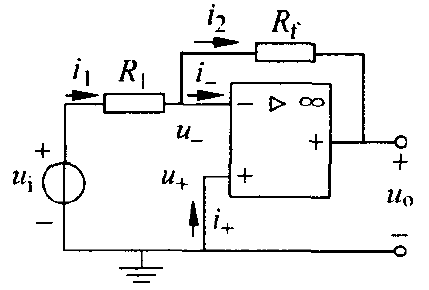
\includegraphics[height=100pt]{assets/3/反向比例放大器.png}
    \caption{\bfseries 同相比例放大器}
\end{subfigure}\begin{subfigure}[t]{0.4\textwidth}\centering
    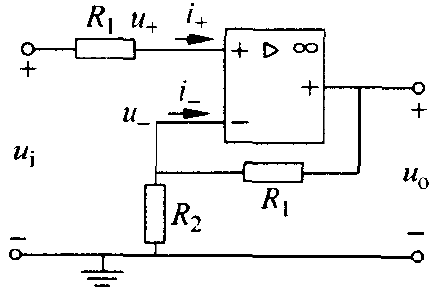
\includegraphics[height=100pt]{assets/3/同相比例放大器.png}
    \caption{\bfseries 反向比例放大器}
\end{subfigure}
\caption{\bfseries 讲义题 2-19}
\end{figure}

\section{讲义题 2-20}
\textbf{(a)} 由 KVL 有:
\begin{equation}
\begin{cases}
    u_1 = R_2(i_1 - i_2) \\
    u_2 = R_1 i_2 
\end{cases}\Longrightarrow  
\begin{cases}
    i_1 = \frac{1}{R_2}u_1 + \frac{1}{R_1}u_2 \\ 
    i_2 = \frac{1}{R_1}u_2
\end{cases},\ 
\boldsymbol{G} = 
\begin{bmatrix}
    \frac{1}{R_2} & \frac{1}{R_1} \\ 
    \frac{1}{R_1} & 0
\end{bmatrix}
\end{equation}

\textbf{(b)} 由 KVL, KCL 有:
\begin{equation}
\begin{cases}
    u_1 = R_1\left( i_1 - \frac{u_1 - u_2}{R_2} \right)\\
    u_2 = R_1 \left( i_2 + \frac{u_1 - u_2}{R_2} \right)
\end{cases}\Longrightarrow  
\begin{cases}
    i_1 = \left( \frac{1}{R_1} + \frac{1}{R_2} \right)u_1 - \frac{1}{R_2}u_2 \\ 
    i_2 =  - \frac{1}{R_2}u_1  + \left( \frac{1}{R_1} + \frac{1}{R_2} \right)u_2\\ 
\end{cases},\ 
\boldsymbol{G} = 
\begin{bmatrix}
    \frac{1}{R_1} + \frac{1}{R_2} & -\frac{1}{R_2} \\ 
    -\frac{1}{R_2} & \frac{1}{R_1} + \frac{1}{R_2}
\end{bmatrix}
\end{equation}

\begin{figure}[H]\centering
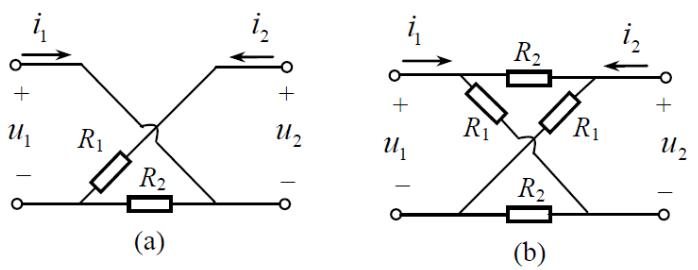
\includegraphics[width=0.7\textwidth]{assets/3/image (8).jpg}
\caption{\bfseries 讲义题 2-20}\label{讲义题 2-20}
\end{figure}

\section{仿真 2-1}

\subsection{单 OPA 实现电压运算}

电路如图 \ref{单 OPA 实现 电压运算} (a) 所示,接线端示意图见图 \ref{单 OPA 实现 电压运算} (b)。

\begin{figure}[H]\centering
\begin{subfigure}[t]{0.43\textwidth}\centering
    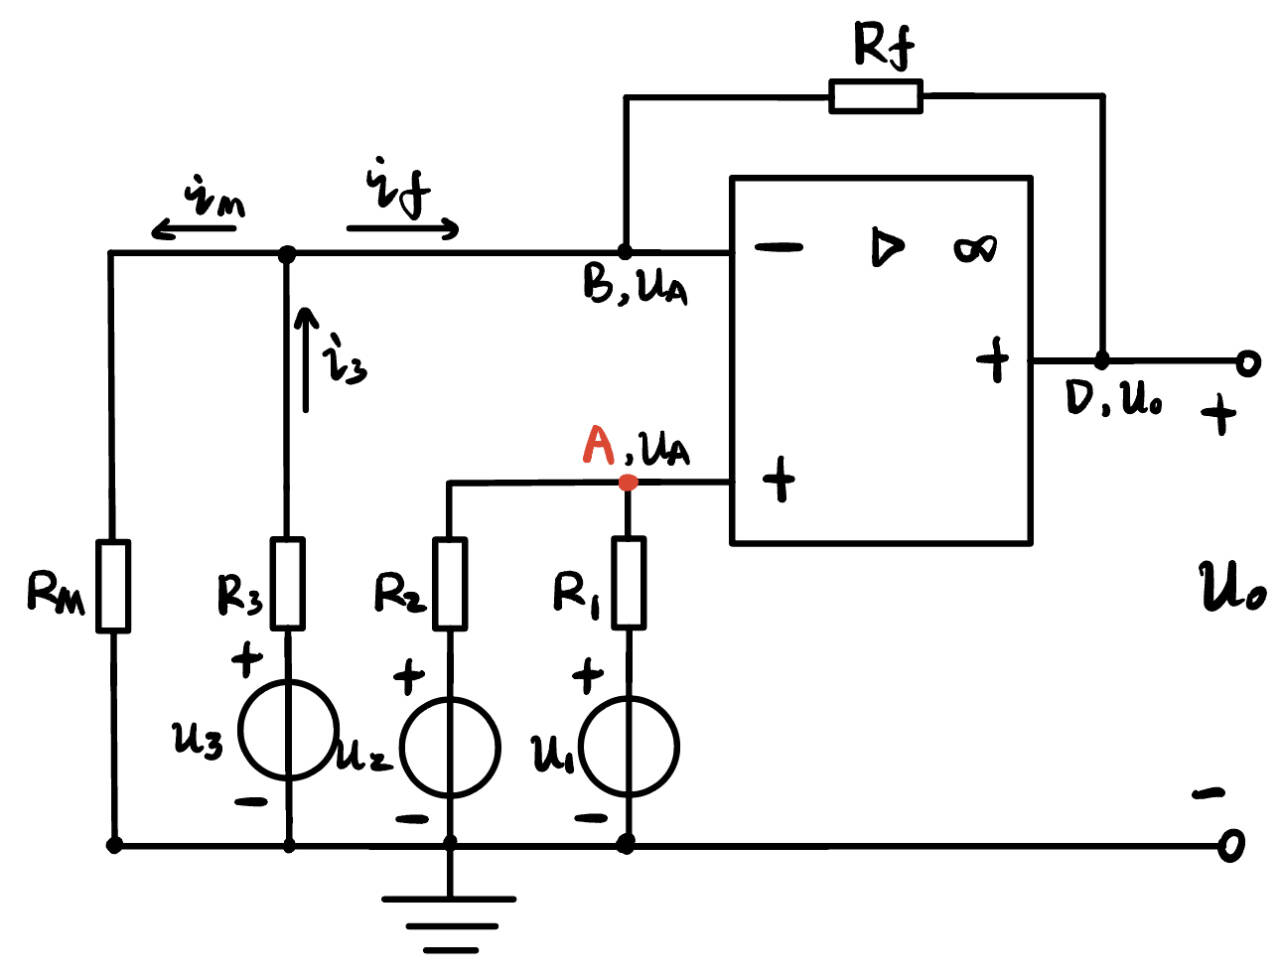
\includegraphics[height=150pt]{assets/3/单OPA.png}
    \caption{\bfseries 电路示意图 }
\end{subfigure}\begin{subfigure}[t]{0.43\textwidth}\centering
    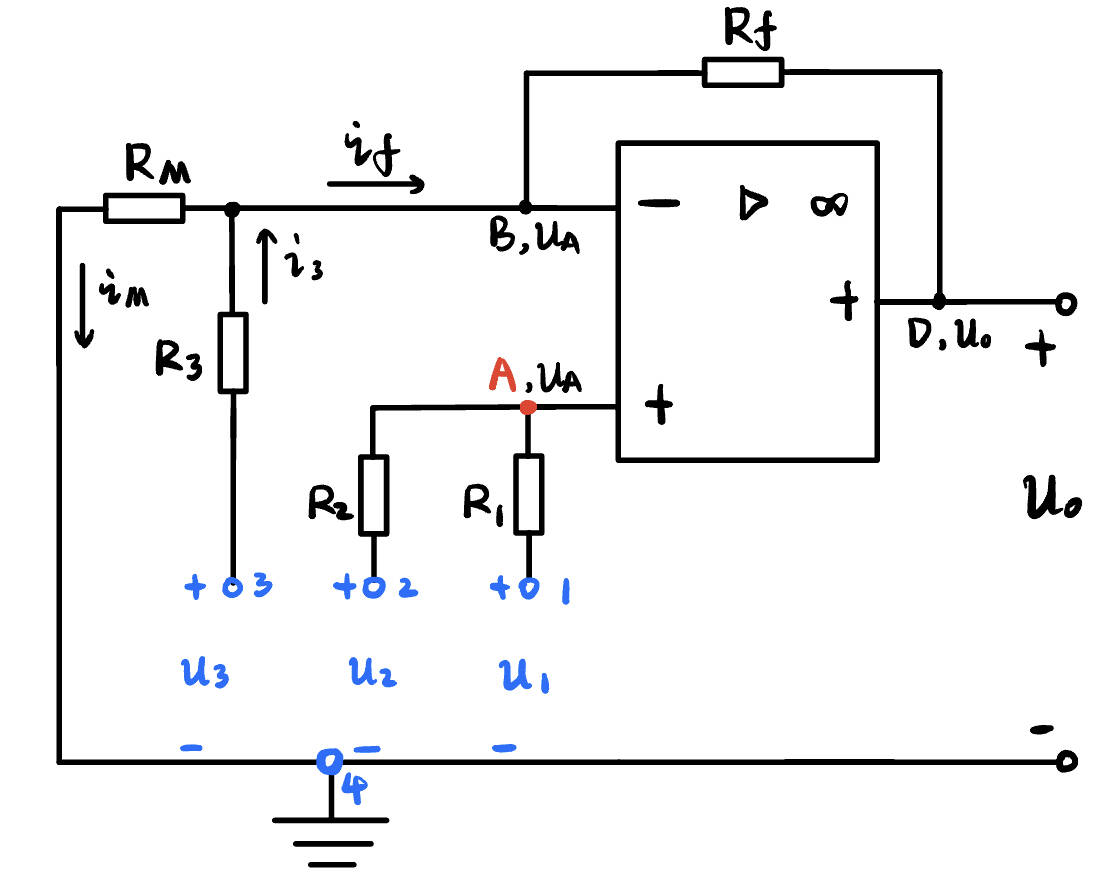
\includegraphics[height=150pt]{assets/3/单OPA接线端.png}
    \caption{\bfseries 接线端示意图 }
\end{subfigure}
\caption{\bfseries 单 OPA 实现 电压运算 }\label{单 OPA 实现 电压运算}
\end{figure}

下面分析其输出特性。由虚断,在 $u_1$ 和 $u_2$ 构成的回路中,设正向流经 $u_2$ 的电流为 $i_2$,则有:
\begin{equation}
i_2 = \frac{u_2 - u_1}{R_1+R_2}
\Longrightarrow  
u_A = u_2 - i_2R_2 = \frac{R_2u_1 + R_1u_2}{R_1 + R_2}
\end{equation}
由虚短,B 点的电势也为 $u_A$,于是:
\begin{equation}
i_3 = \frac{u_3 - u_A}{R_3},\ i_M = \frac{u_A}{R_M} \Longrightarrow  i_f = i_3 - i_M = \frac{u_3 - u_A}{R_3} - \frac{u_A}{R_M} = \frac{u_3}{R_3} - (\frac{1}{R_3} + \frac{1}{R_M})u_A
\end{equation}
由虚断和 KVL:
\begin{equation}
u_o = u_A - i_fR_f = u_A - \frac{R_f}{R_3}u_3 + (\frac{R_f}{R_3} + \frac{R_f}{R_M})u_A = \left( 1 +  \frac{R_f}{R_3} + \frac{R_f}{R_M}\right)u_A - \frac{R_f}{R_3}u_3
\end{equation}
将 $u_A$ 的表达式代入,最终得到:
\begin{equation}
\boxed{
    u_o = \left( 1 +  \frac{R_f}{R_3} + \frac{R_f}{R_M}\right)\frac{1}{\frac{R_1}{R_2} + 1}u_1 
    + \left( 1 +  \frac{R_f}{R_3} + \frac{R_f}{R_M}\right)\frac{\frac{R_1}{R_2}}{\frac{R_1}{R_2} + 1}u_2
    - \frac{R_f}{R_3}u_3
}
\end{equation}
我们需要 $u_1,u_2,u_3$ 前的系数分别为 3, 2, -0.5,于是有:
\begin{equation}
\begin{cases}
    \left( 1 +  \frac{R_f}{R_3} + \frac{R_f}{R_M}\right)\frac{1}{\frac{R_1}{R_2} + 1} = 3 \vspace*{5pt}\\ 
    \vspace*{5pt}
    \left( 1 +  \frac{R_f}{R_3} + \frac{R_f}{R_M}\right)\frac{\frac{R_1}{R_2}}{\frac{R_1}{R_2} + 1} = 2 \\ 
    -\frac{R_f}{R_3} = -0.5
\end{cases}
\Longrightarrow 
\begin{cases}
    R_1 = \frac{2}{3}R_2 &,\ R_2 > 0\\ 
    R_3 = 2R_f,\ R_M = \frac{2}{7}R_f &,\ R_f >0\\
\end{cases}
\end{equation}
为了保持 OPA 的理想性,我们应选择 $\KO$ 量级的电阻,同时,为了降低电路的整体功率,减少消耗,电阻阻值应该尽量大。综合下来,不妨选取 $R_2 = 6 \KO,\ R_f = 3.5 \KO$,此时所有电阻阻值为:
\begin{equation}
R_1 = 4\KO,\ R_2 = 6\KO,\ R_3 = 7\KO,\ R_M = 1\KO,\ R_f = 3.5\KO
\end{equation}

如图 \ref{单 OPA 实现电压运算仿真} (a),在 Multisim 中进行仿真,得到的结果如下表所示:

% \usepackage[longtable]{multirow}
% \usepackage{longtable}


\begin{longtable}{|c|c|c|c|c|c|c|c|c|c|c|c|c|} 
    \hline
    \multirow{3}{*}{项目} & \multicolumn{3}{c|}{1} & \multicolumn{3}{c|}{2} & \multicolumn{3}{c|}{3} & \multicolumn{3}{c|}{4}  \\* 
    \cline{2-13}
                      & $x,\ u_1$ & $y,\ u_2$ & $z,\ u_3$  & $x,\ u_1$ & $y,\ u_2$ & $z,\ u_3$               &  $x,\ u_1$ & $y,\ u_2$ & $z,\ u_3$             &  $x,\ u_1$ & $y,\ u_2$ & $z,\ u_3$              \\* 
    \cline{2-13}
                      & 1     & 1     & 1      & 1 & 3 & 2              & -2 & 2 & 0             & 3 & 3 & 2               \endfirsthead 
    \hline
    理论输出 $(\mathrm{V})$             & \multicolumn{3}{c|}{$3+2-0.5 = 4.5$}  & \multicolumn{3}{c|}{$3+6-1=8$}  & \multicolumn{3}{c|}{$-6+4-0 = -2$}  & \multicolumn{3}{c|}{$9+6-1=14$}   \\ 
    \hline
    仿真输出 $(\mathrm{V})$     & \multicolumn{3}{c|}{4.50}  & \multicolumn{3}{c|}{8.00}  & \multicolumn{3}{c|}{-2.00}  & \multicolumn{3}{c|}{10.494}   \\
    \hline
\end{longtable}

\begin{figure}[H]\centering
\begin{subfigure}[t]{0.45\textwidth}\centering
    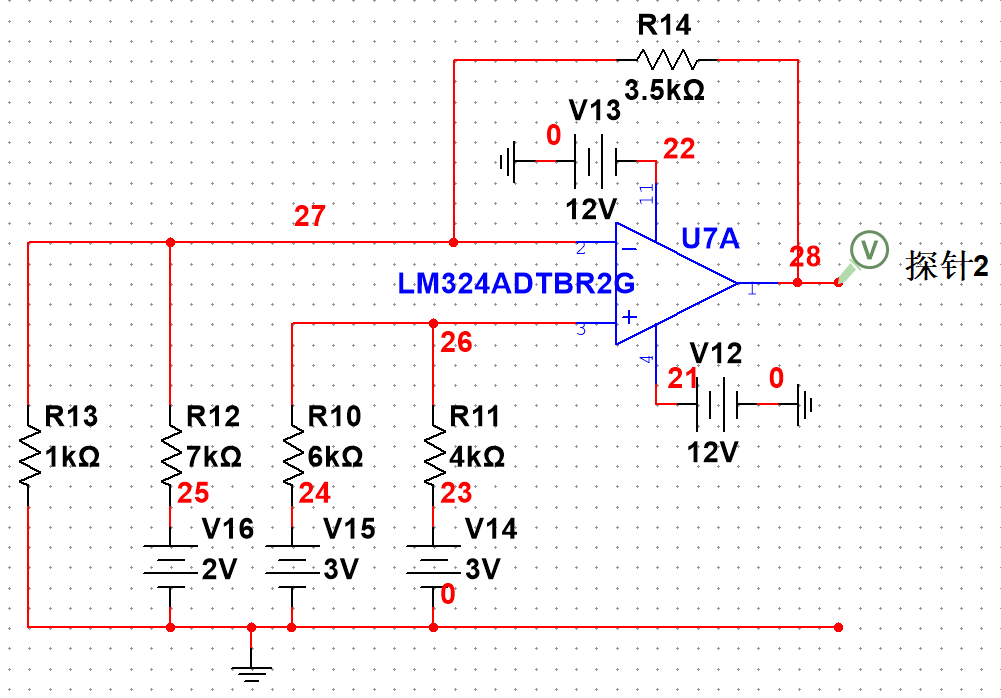
\includegraphics[height=130pt]{assets/3/8a5141629bce86a4810852d0002e5180.png}
    \caption{\bfseries 单 OPA 实现电压运算 }
\end{subfigure}\begin{subfigure}[t]{0.53\textwidth}\centering
    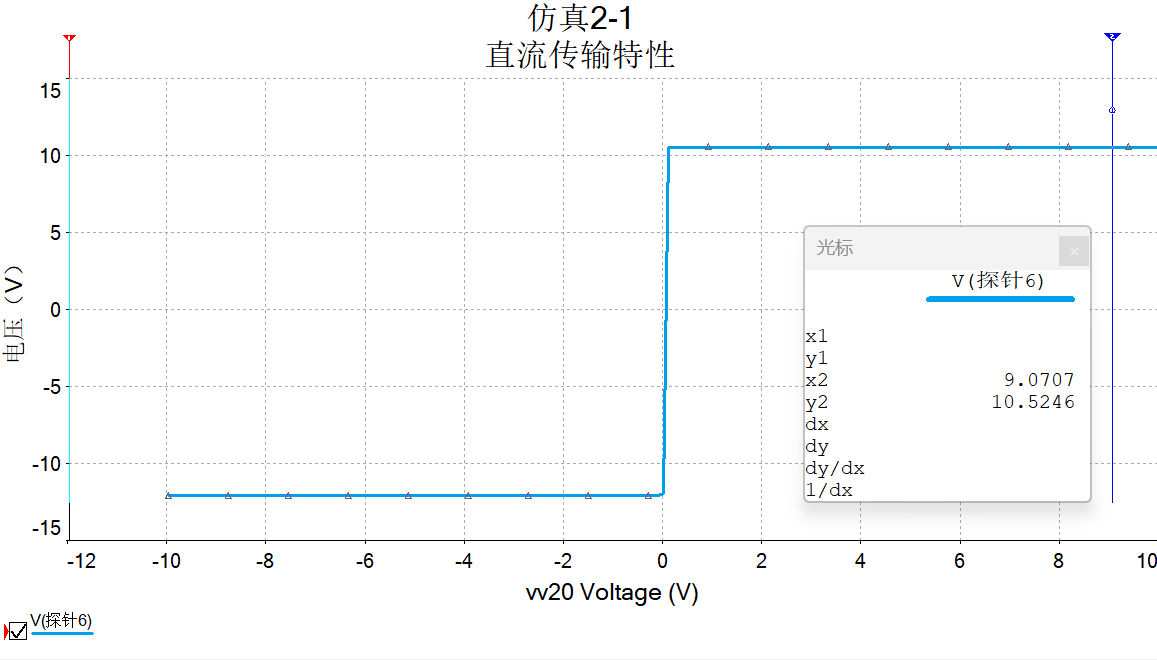
\includegraphics[height=130pt]{assets/3/OPA饱和电流.png}
    \caption{\bfseries OPA 饱和电压 }
\end{subfigure}
\caption{\bfseries 仿真电路图与 OPA 饱和电压 }\label{单 OPA 实现电压运算仿真}
\end{figure}

由表可见,除了最后一组数据,仿真结果与理论结果完全一致。最后一组之所以不同,是因为输出电压 $u_o$ 超出了此 OPA 的饱和电压 $U_{\text{sat}}$,导致输出电压 $u_o = U_{\text{sat}} = 10.494 \mathrm{V}$。如图 \ref{单 OPA 实现电压运算仿真} (b) 所示,此 OPA (LM324ADTBR2G) 的饱和电压为 $10.525 \mathrm{V}$,与解释相符。具体仿真时的结果见图 \ref{一个图}。

\begin{figure}[H]\centering
\begin{subfigure}[t]{0.48\textwidth}\centering
    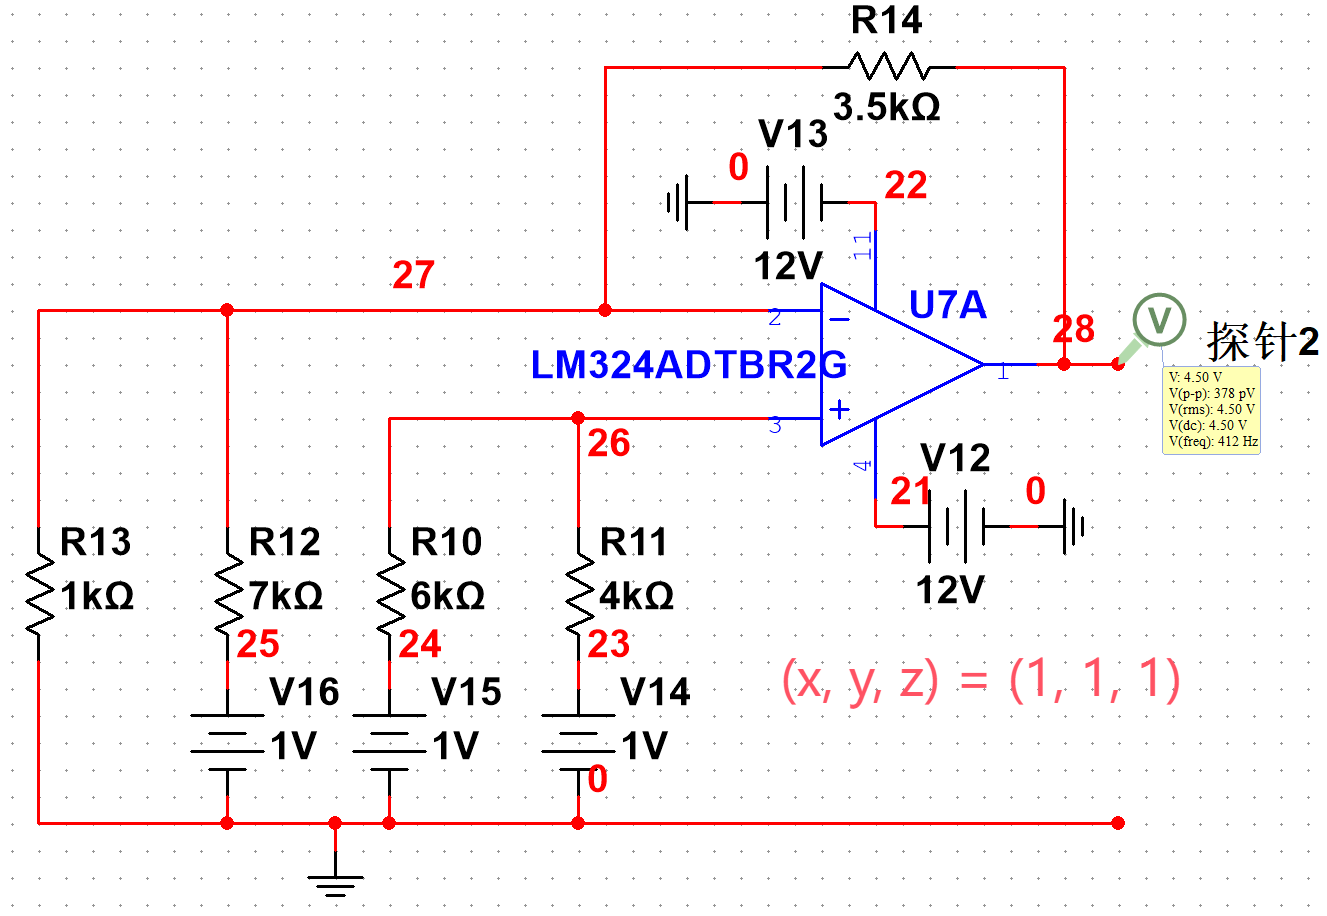
\includegraphics[height=145pt]{assets/3/111.png}
    \caption{\bfseries $(x,y,z) = (1,1,1)$ }
\end{subfigure}\begin{subfigure}[t]{0.48\textwidth}\centering
    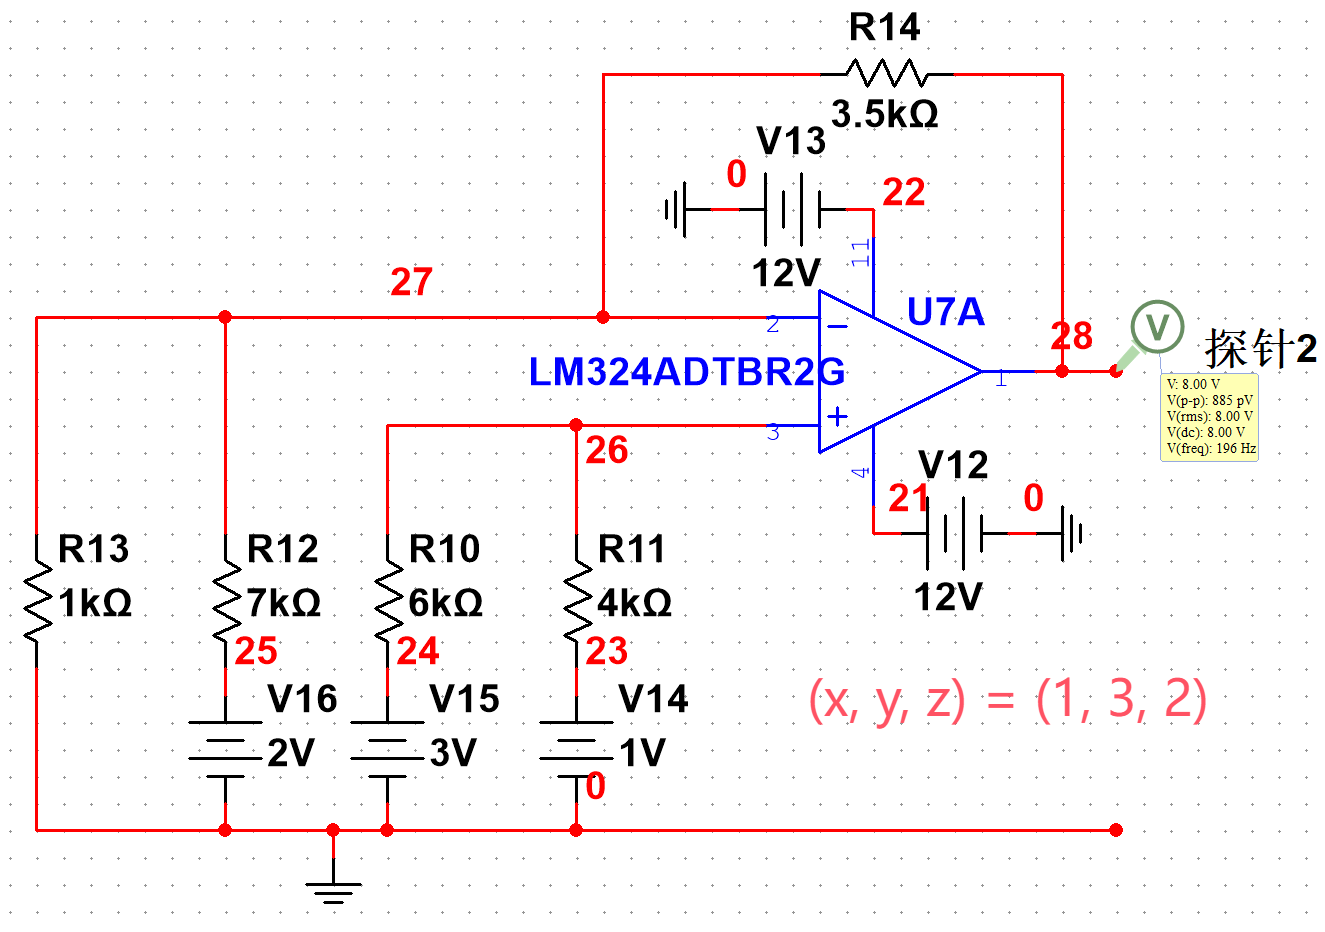
\includegraphics[height=145pt]{assets/3/132.png}
    \caption{\bfseries $(x,y,z) = (1,3,2)$ }
\end{subfigure}
\begin{subfigure}[t]{0.48\textwidth}\centering
    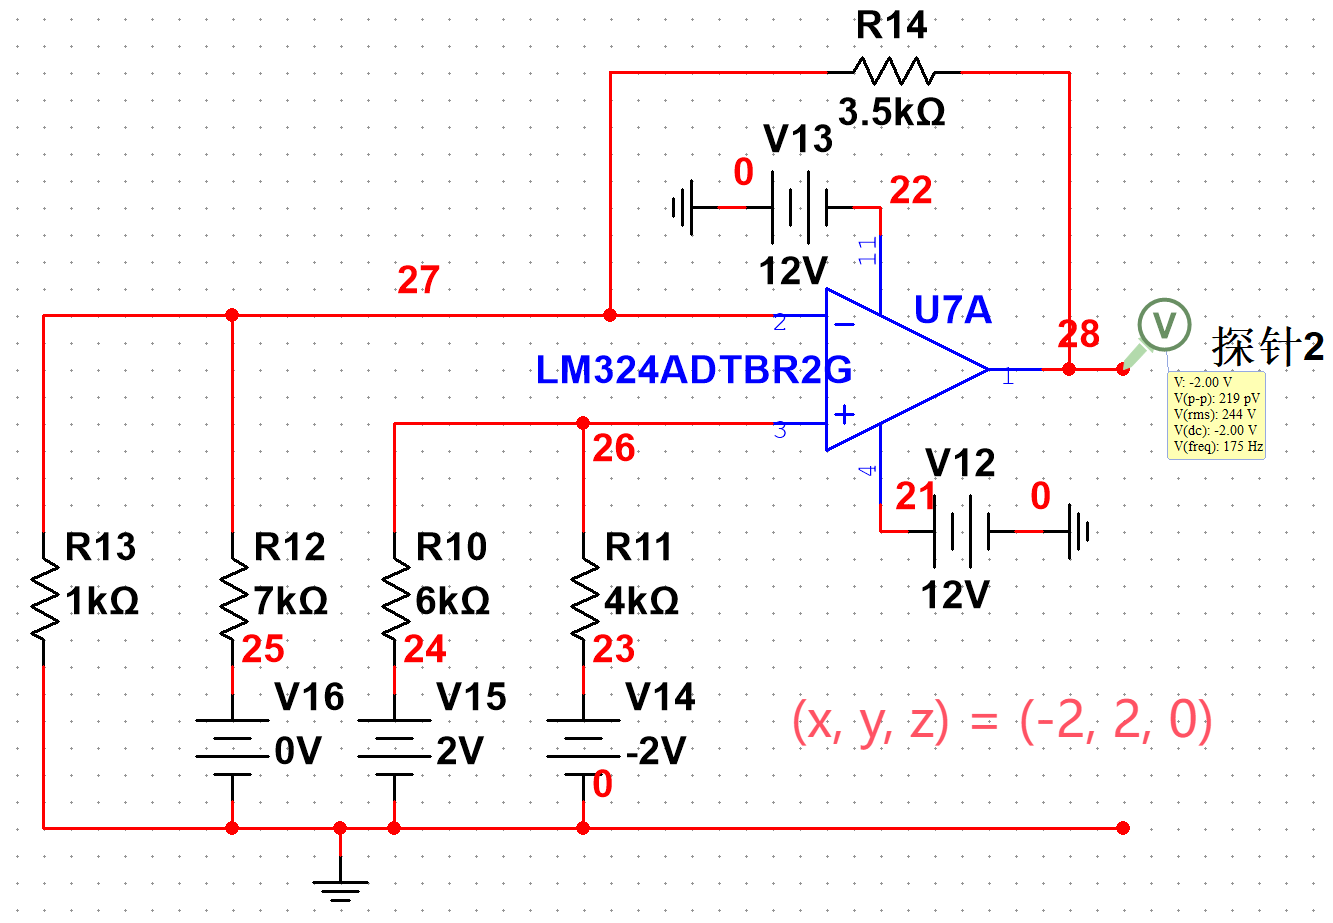
\includegraphics[height=145pt]{assets/3/91f965079537c7c35944182511dce291.png}
    \caption{\bfseries $(x,y,z) = (-2,2,0)$ }
\end{subfigure}\begin{subfigure}[t]{0.48\textwidth}\centering
    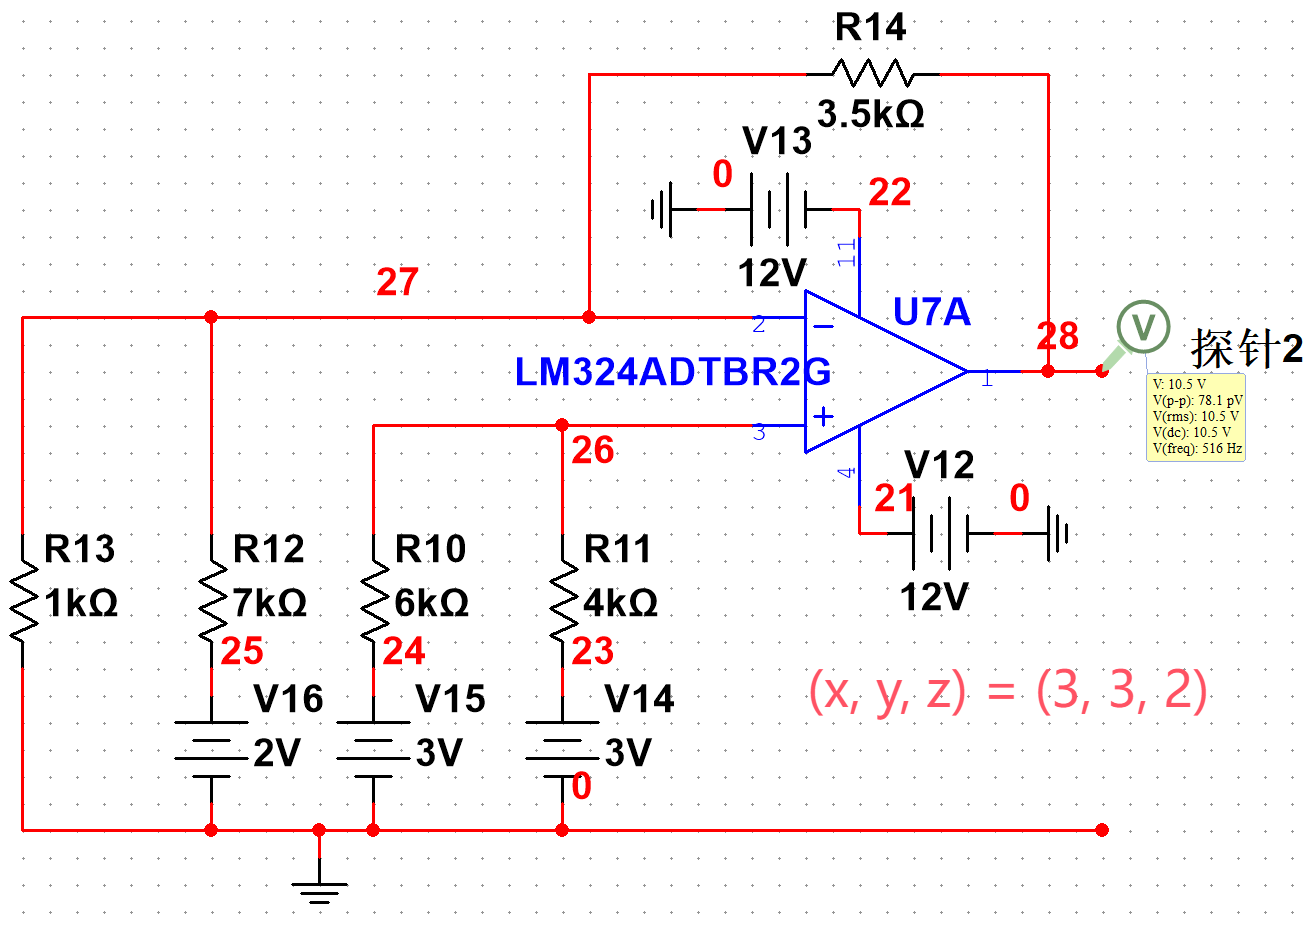
\includegraphics[height=145pt]{assets/3/def5c414621689edf67e4afb5251cf4a.png}
    \caption{\bfseries $(x,y,z) = (3,3,2)$ }
\end{subfigure}
\caption{\bfseries 仿真具体结果图 }\label{一个图}
\end{figure}


\subsection{一些失败的例子}
注意到,减法器是在反相加法器的基础上,串联入电压源(和电阻)改变了 $u_+$ 端的电压。这样,在最终的输出电压 $u_o$ 中,$u_-$ 端的电源电压会带负号,$u_+$ 端的电源电压带正号。用类似的思想,我们可以对减法器进行改造,最终仅用一个 OPA 便实现 $3x+2y-0.5z$ 的电压运算。

一种方法是向 $u_+$ 端再串联一个电压源,使得输出 $u_o$ 中两正一负,然后通过电阻值来调整系数,但是,这样不满足接线端的要求(三正一共地)。另一种方法是向 $u_-$ 端再并联一个电压源,使得输出 $u_o$ 中两负一正($-u_1,\ -u_2,\ +u_3$),最后通过电阻值来调整系数,但是,这样得到的是两负一正而不是两正一负,虽满足了接线端要求,却不是我们需要的结果。

其实,我们只需要向 $u_+$ 端的电压源再并联一个电压源即可,如图所示。下面分析其输出特性。

\begin{figure}[H]\centering
\begin{subfigure}[t]{0.43\textwidth}\centering
    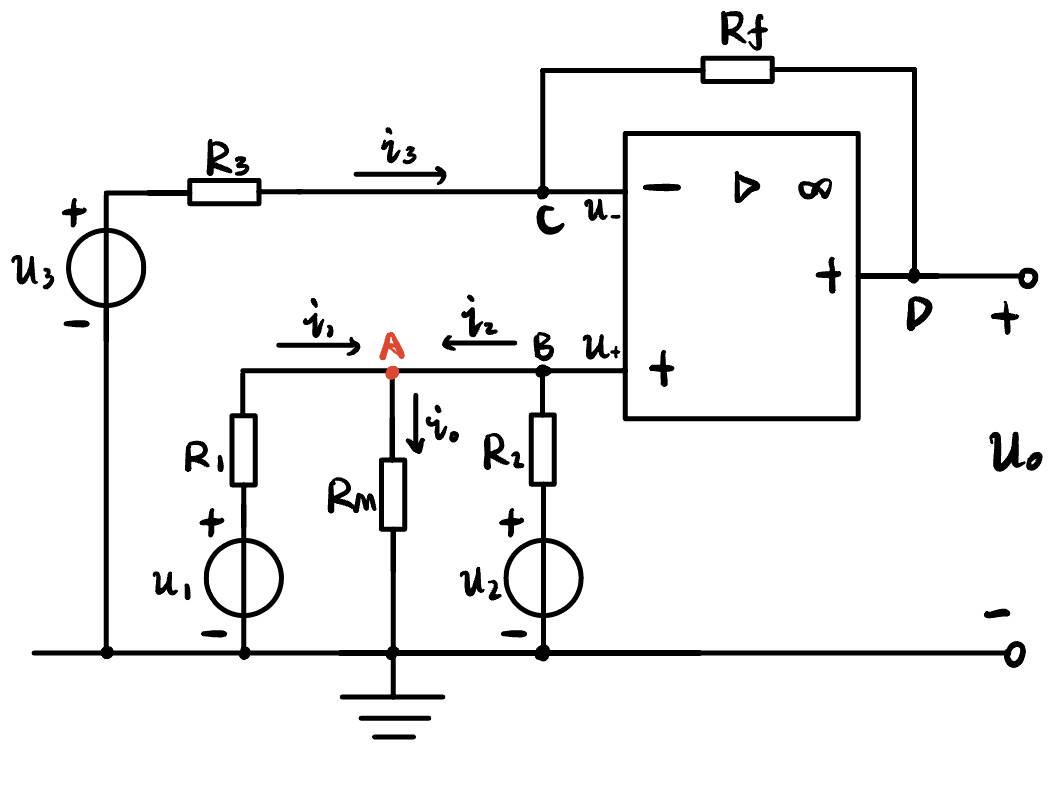
\includegraphics[height=120pt]{assets/3/失败的例子.png}
    \caption{\bfseries 失败的例子 }
\end{subfigure}\begin{subfigure}[t]{0.43\textwidth}\centering
    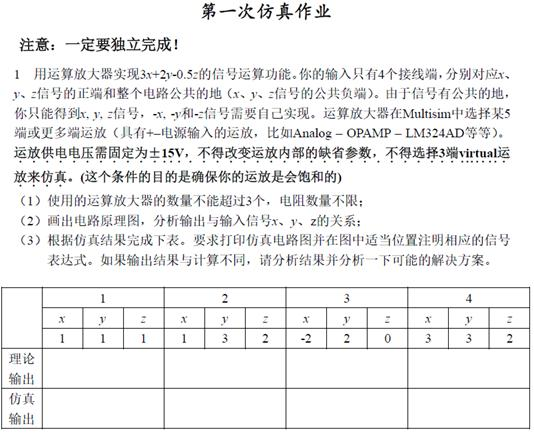
\includegraphics[height=120pt]{assets/3/image (5).jpg}
    \caption{\bfseries 仿真作业 2-1 }
\end{subfigure}
\caption{\bfseries 示意图 }
\end{figure}

在 $u_1, R_1, u_2, R_2 $ 和 $R_M$ 构成的局部电路中,由 KVC:
\begin{gather}
\begin{cases}
    u_1 - R_1i_1 - R_M(i_1 + i_2) = 0 \\
u_2 - R_2i_2 - R_M(i_1 + i_2) = 0
\end{cases}
\Longrightarrow 
\begin{cases}
    i_1 = \frac{(R_2+R_M)u_1 - R_Mu_2}{R_1R_2 +R_1R_M + R_2R_M} \\ 
    i_2 = \frac{(R_1+R_M)u_2 - R_Mu_1}{R_1R_2 +R_1R_M + R_2R_M} \\ 
\end{cases}
\end{gather}
由此得点 A 处的电势 $u_A$:
\begin{equation}
    u_A = \frac{R_2R_Mu_1 + R_1R_Mu_2}{R_1R_2 +R_1R_M + R_2R_M}
\end{equation}
也即点 B 和非反相输入端的电势 $u_+ = u_B = u_A$。由虚短,$u_- = u_+$,可得电流 $i_3$:
\begin{equation}
i_3 = \frac{u_3 - u_-}{R_3} = \frac{1}{R_3}(u_3 - \frac{R_2R_Mu_1 + R_1R_Mu_2}{R_1R_2 +R_1R_M + R_2R_M}) 
\end{equation}
由虚断,经过电阻 $R_f$ 求得 D 点电势,也即输出电压 $u_o$:
\begin{align}
u_o &= u_A - i_3R_f = (1+\frac{R_f}{R_3})u_A - \frac{R_f}{R_3}u_3 
\\
&= (1+\frac{R_f}{R_3})\cdot \frac{\frac{R_M}{R_1}u_1 + \frac{R_M}{R_2}u_2}{1 + \frac{R_M}{R_1} + \frac{R_M}{R_2}} - \frac{R_f}{R_3}u_3
\\ 
&=\frac{1+\frac{R_f}{R_3}}{1 + \frac{R_M}{R_1} + \frac{R_M}{R_2}}
\left( \frac{R_M}{R_1}u_1 + \frac{R_M}{R_2}u_2  \right) - \frac{R_f}{R_3}u_3
\end{align}

最后调整电阻阻值。为了保持 OPA 的理想性,电阻需要在 $\KO$ 量级,令电阻比例如下:
\begin{equation}
\begin{cases}
    \frac{R_f}{R_3} = 0.5 \\ 
    \frac{1+\frac{R_f}{R_3}}{1 + \frac{R_M}{R_1} + \frac{R_M}{R_2}}\cdot \frac{R_M}{R_1} = 3 \\ 
    \frac{1+\frac{R_f}{R_3}}{1 + \frac{R_M}{R_1} + \frac{R_M}{R_2}}\cdot \frac{R_M}{R_2} = 2
\end{cases}\Longrightarrow 
\begin{cases}
    R_f = \frac{1}{2}R_3 \\ 
    R_1 =  -2R_M\\ 
    R_2 = -\frac{4}{3}R_M
\end{cases}
\end{equation}
显然,这不可能实现,舍弃。



\section{仿真 2-2}

仿真电路如图 \ref{负电阻仿真} (a) 所示,对输入电压进行参数扫描,输出通过电压源的电流,得到图 \ref{负电阻仿真} (b)。这里需要注意,在 Multisim 中,电流的参考方向始终是高电势指向低电势(包括电压源),因此,仿真输出中的 I(V11) 是从上往下通过 V11 的电流(而不是从下至上),电压源 V11 的实际电流为 $i = -I(V11)$。

\begin{figure}[H]\centering
\begin{subfigure}[t]{0.47\textwidth}\centering
    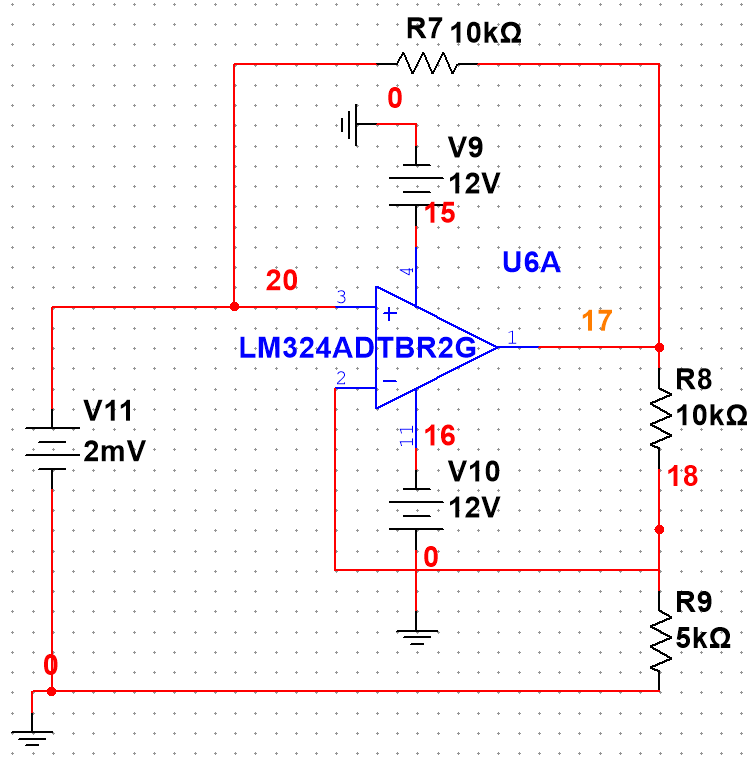
\includegraphics[height=140pt]{assets/3/0649949f48a11f77b47f406012e3f7a8.png}
    \caption{\bfseries 负电阻仿真电路 }
\end{subfigure}\begin{subfigure}[t]{0.5\textwidth}\centering
    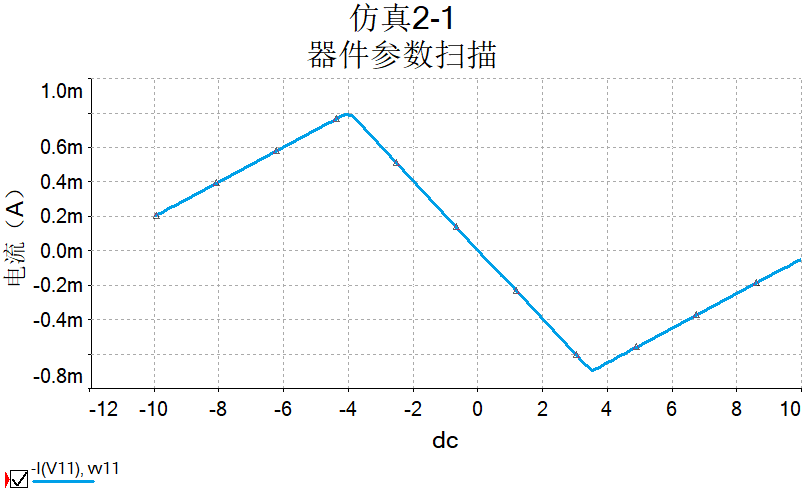
\includegraphics[height=140pt]{assets/3/83d7126e6d74b406acb4bbc94900f2c6.png}
    \caption{\bfseries $I$(纵轴)$U$(横轴)关系 }
\end{subfigure}
\caption{\bfseries 负电阻仿真 }\label{负电阻仿真}
\end{figure}

简记电压源 V11 的电压为 $u$,继续仿真输出电压 $u_o$ 关于输入电压 $u$ 的变化,将数据导出后在 Matlab 中绘制曲线,如图 \ref{仿真结果分析} (a)。再将 $I-U$ 关系转化为 $U-I$ 关系,如图 \ref{仿真结果分析} (b)。可以发现,在线性工作区内,电路表现为负阻。而线性区外的两段折线位于 OPA 的饱和区,此时 $u_o$ 始终为饱和电压,电路呈现正电阻,且阻值为:
\begin{equation}
\begin{cases}
    i = \frac{u - U_{\text{sat}}}{R_1} &, u > 3.54\ \mathrm{V} \\ 
    i = \frac{u + U_{\text{sat}}}{R_1} &, u < -4.05 \ \mathrm{V} \\ 
\end{cases}\Longrightarrow 
R_{\text{sat}} = R_1 = 10 \KO
\end{equation}
这与图 \ref{仿真结果分析} (b) 中曲线的斜率是相符的。而在线性区,负电阻 $R = -\frac{10 \KO}{10 \KO} \cdot 5 \KO = - 5 \KO$,这也是符合的。

\begin{figure}[H]\centering
\begin{subfigure}[t]{0.52\textwidth}\centering
    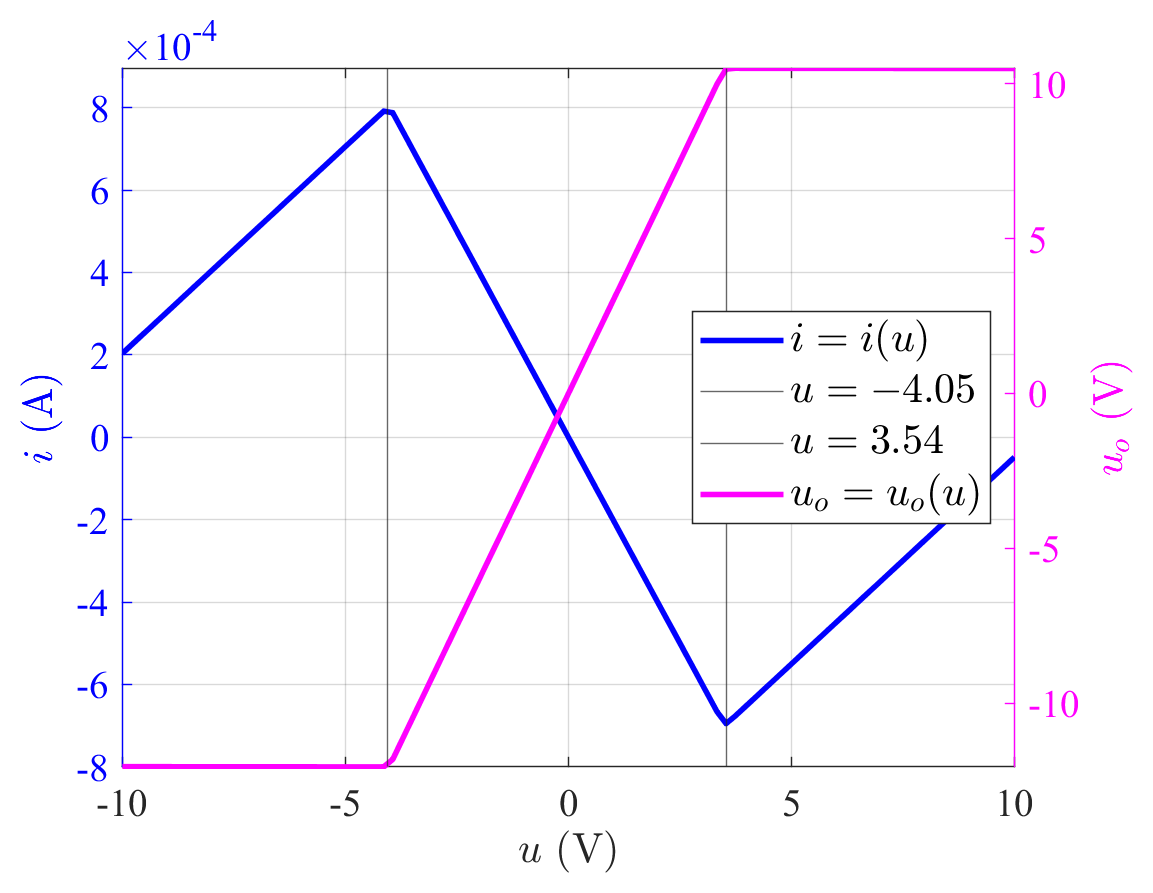
\includegraphics[height=190pt]{assets/3/2024-09-13_01-13-08.png}
    \caption{\bfseries $u_o$ 与 $i$ 关于 $u$ 的变化}
\end{subfigure}\begin{subfigure}[t]{0.47\textwidth}\centering
    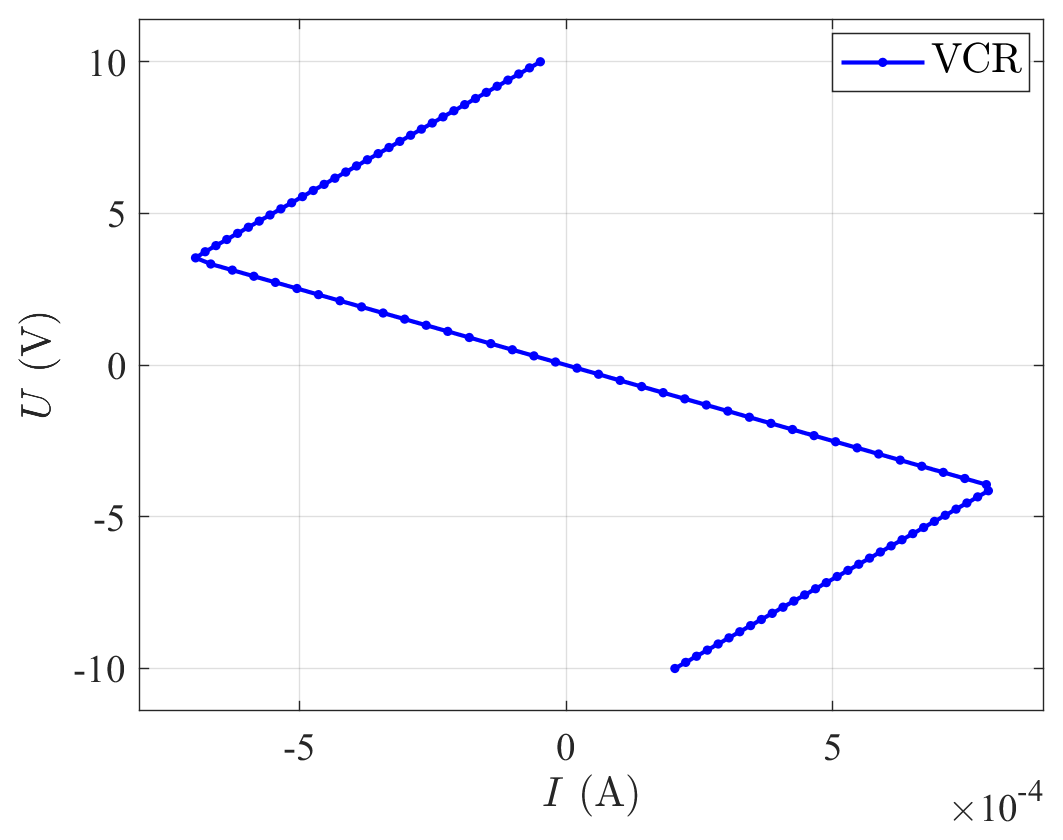
\includegraphics[height=180pt]{assets/3/2024-09-13_01-13-52.png}
    \caption{\bfseries $U$-$I$ 关系(VCR)}
\end{subfigure}
\caption{\bfseries 仿真结果分析 }\label{仿真结果分析}
\end{figure}

%在负电阻中,OPA 输出电压 $u_o$:
%\begin{equation}
%u_o = \left(1 + \frac{R_2}{R}\right)u_i
%\end{equation}
%由图 \ref{单 OPA 实现电压运算仿真} (b) 可知,我们选择的 OPA 饱和电压 $U_{\text{sat}} = 10.525\ V$,输入电压线性区约为 [0 mV, 100 mV]。因此,当 $u_i < $ 或 $u_i >$ 时,OPA 工作在饱和区,此时 $u_o = \pm U_{\text{sat}}$ 为定值,且虚短不再成立,电流 $i_1$:
%\begin{equation}
%i_1 = \frac{u_1 - u_o}{R_1} = 
%\begin{cases}
%    \frac{u_1 - U_{\text{sat}}}{R_1} &, u_1 > \\ 
%    \frac{u_1 + U_{\text{sat}}}{R_1} &, u_1 < \\ 
%\end{cases}
%\end{equation}
%\begin{figure}[H]\centering
%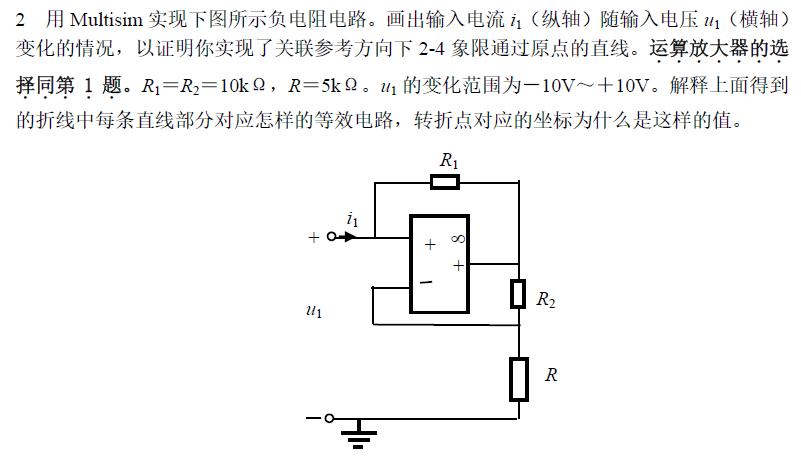
\includegraphics[width=0.45\textwidth]{assets/3/ee57b549a02999b0856af303ac0e8510.jpg}
%\caption{\bfseries 第一次仿真作业 (2)}\label{第一次仿真作业 (2)}
%\end{figure}



\chapter{第二章}\thispagestyle{fancy}

\section{对于正入射的情况,写出菲涅尔公式}

菲涅尔公式如下:

\begin{table}[H]
    \centering
    \begin{tabular}{|c|c|c|c|c|} 
    \hline
    类型 & \multicolumn{2}{c|}{振幅反射系数 $r$} & \multicolumn{2}{c|}{振幅透射系数 $t$ }  \\ 
    \hline
    s 波 & $\displaystyle r_s = \frac{n_i\cos \theta_i - n_t \cos \theta_t}{n_i\cos \theta_i + n_t \cos \theta_t} $ & $\displaystyle  - \frac{\sin (\theta_i - \theta_t) }{\sin (\theta_i + \theta_t)}$ & $\displaystyle t_s  = \frac{2n_i \cos \theta_i}{n_i\cos \theta_i + n_t \cos \theta_t} $ &   $\displaystyle  + \frac{2 \sin \theta_t \cos \theta_i}{\sin (\theta_i + \theta_t)}$   \\ 
    \hline
    p 波 & $\displaystyle r_p = \frac{n_t\cos \theta_i - n_i \cos \theta_t}{n_t\cos \theta_i + n_i \cos \theta_t} $ &     $ \displaystyle  + \frac{\tan (\theta_i - \theta_t)}{\tan (\theta_i + \theta_t)} $  &  $\displaystyle t_p  = \frac{2n_i \cos \theta_i}{n_i\cos \theta_t + n_t \cos \theta_i} $ &   $\displaystyle + \frac{2 \sin \theta_t \cos \theta_i}{\sin (\theta_i + \theta_t) \cos (\theta_i - \theta_t)}$                  \\
    \hline
    \end{tabular}
\end{table}

正入射时,$\theta_i = \theta_t = 0$,于是有:
\begin{gather}
    r_p = (-r_s)  = \frac{n_t - n_i}{n_t + n_i},\quad t_p = t_s = \frac{2n_i}{n_i + n_t} \\ 
    F = R_s = R_p = \left( \frac{n_t - n_i}{n_t + n_i} \right)^2
\end{gather}


不妨作出相关的图像,图 \ref{振幅系数随入射角的变化} 是 s 波、p 波振幅系数关于入射角 $\theta_i$ 的变化情况\footnote{源码见附录 \ref{图振幅系数随入射角的变化源码}}。

\begin{figure}[H]\centering
\begin{subfigure}[t]{0.49\textwidth}\centering
    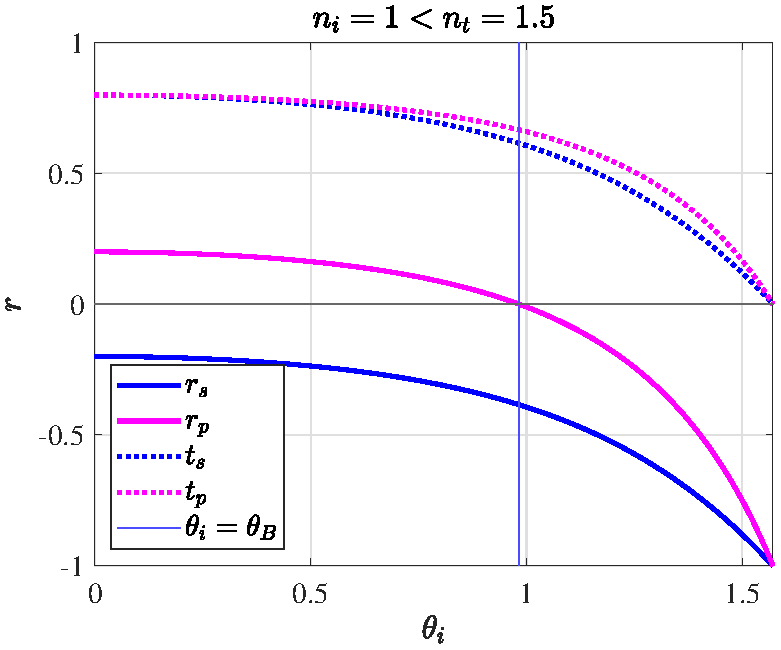
\includegraphics[height=180pt]{assets/2/2024-09-15_10-53-31.pdf}
    \caption{\bfseries 由空气入射玻璃($n_i = 1,\ n_t = 1.5$) }
\end{subfigure}
\begin{subfigure}[t]{0.49\textwidth}\centering
    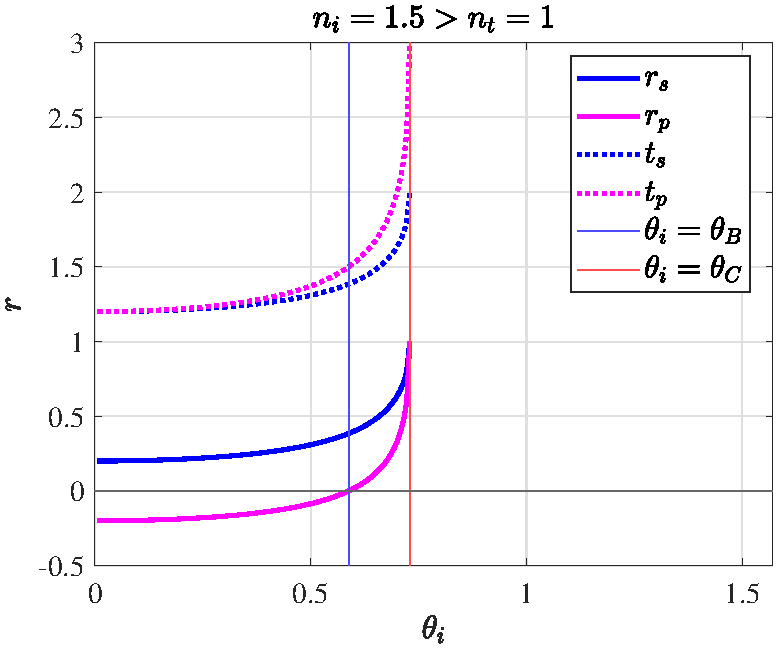
\includegraphics[height=180pt]{assets/2/2024-09-15_10-53-27.pdf}
    \caption{\bfseries 由玻璃入射空气($n_i = 1.5,\ n_t = 1$) }
\end{subfigure}
\caption{\bfseries 振幅系数 $r$ 随入射角 $\theta_i$ 的变化 }\label{振幅系数随入射角的变化}
\end{figure}


\section{一自然光以 Brewster Angle 入射到空气中的一块玻璃,已知功率透射率为 0.86。}
\begin{enumerate}
\item \textbf{求功率的反射率:}

$T = 0.86$,由能量守恒,功率反射率 $R = 0.14$。
\item \textbf{若输入为 1000 W,求透射光 s 分量上的功率}

光束为自然光,因此 s 分量和 p 分量的功率相同,都为 500 W。先求解入射角 $\theta_i$,由菲涅尔定理和能量关系:
\begin{equation}
R =  \frac{1}{2}(R_s + R_p),\  R_s =  \left[ \frac{ \cos \theta_i - \sqrt{n_{ti}^2 - \sin^2 \theta_i} }{\cos \theta_i + \sqrt{n_{ti}^2 - \sin^2 \theta_i}} \right]^2,\ R_p = \left[ \frac{ n_{ti}^2\cos \theta_i - \sqrt{n_{ti}^2 - \sin^2 \theta_i} }{n_{ti}^2\cos \theta_i + \sqrt{n_{ti}^2 - \sin^2 \theta_i}} \right]^2
\end{equation}
其中 $n_i = 1$,$n_t = 1.5$,因此 $n_{ti} = 1.5$,代入即得:
\begin{equation}
    \left[ \frac{ \cos \theta_i - \sqrt{1.5^2 - \sin^2 \theta_i} }{\cos \theta_i + \sqrt{1.5^2 - \sin^2 \theta_i}} \right]^2 + \left[ \frac{ 1.5^2\cos \theta_i - \sqrt{1.5^2 - \sin^2 \theta_i} }{1.5^2\cos \theta_i + \sqrt{1.5^2 - \sin^2 \theta_i}} \right]^2 = 2\times0.14
\end{equation}
用 Matlab 解此非线性方程组\footnote{源码见附录 \ref{公式解入射角源码}},得到入射角 $\theta_i$ 和其它参量:
\begin{gather}\label{解入射角}
\begin{matrix}
    \theta_i =  1.173220\ \ \mathrm{rad}  = 67.220559^\circ \\
    R = 0.14,\quad   R_s = 0.256933,\    R_p = 0.023067 \\ 
    T = 0.86,\quad   T_s = 0.743067,\    T_p = 0.976933 
\end{matrix}
\end{gather}

\end{enumerate}

\section{光束垂直入射到玻璃-空气界面,玻璃折射率 1.5,求出能量反射率和透射率}

$\theta_i = 0$ 时,由菲涅尔定律和能量关系,有:
\begin{gather}
    R =  \frac{1}{2}(R_s + R_p),\quad  T = 1 - R\\ 
    R_s =  \left[ \frac{ \cos \theta_i - \sqrt{n_{ti}^2 - \sin^2 \theta_i} }{\cos \theta_i + \sqrt{n_{ti}^2 - \sin^2 \theta_i}} \right]^2 = \left[ \frac{1 - n_{ti}}{1 + n_{ti}} \right]^2,\ R_p = \left[ \frac{ n_{ti}^2\cos \theta_i - \sqrt{n_{ti}^2 - \sin^2 \theta_i} }{n_{ti}^2\cos \theta_i + \sqrt{n_{ti}^2 - \sin^2 \theta_i}} \right]^2 =  \left[ \frac{n_{ti}^2 - n_{ti}}{n_{ti}^2 + n_{ti}} \right]^2
\end{gather}
由空气入射玻璃时,$n_{ti} = 1.5$,由玻璃入射空气时,$n_{ti} = \frac{2}{3}$,代入得到:
\begin{gather*}
\text{空气入射玻璃: }\ R = 0.04,\quad  T = 0.96 \\ 
\text{玻璃入射空气: }\ R = 0.04,\quad  T = 0.96 
\end{gather*}
也即无论从哪边入射,能量反射率和透射率分别为 0.04 和 0.96.



\nocite{*}
\bibliography{re}
\thispagestyle{fancy} 
\addcontentsline{toc}{chapter}{参考文献}


% ------------------------------------------------------------ %
% >> ------------------------ 附录 ------------------------ << %

\newpage
\appendix
% chapter 标题自定义设置
\titleformat{\chapter}[hang]{\normalfont\huge\bfseries\centering}{}{20pt}{}
\titlespacing*{\chapter}{0pt}{-25pt}{8pt} % 控制上方空白的大小
% section 标题自定义设置 
\titleformat{\section}[hang]{\normalfont\centering\Large\bfseries}{\thesection}{8pt}{}

% 附录 A
\chapter*{附录 A. Matlab 代码}\addcontentsline{toc}{chapter}{附录 A. Matlab 代码}   
\thispagestyle{fancy} 
\setcounter{section}{0}   
\renewcommand\thesection{A.\arabic{section}}   
\renewcommand{\thefigure}{A.\arabic{figure}} 
\renewcommand{\thetable}{A.\arabic{table}}

\section{图 \ref{振幅系数随入射角的变化} 源码}\label{图振幅系数随入射角的变化源码}
\begin{matlablisting}
%%%%%%%%%% 空气入射玻璃 %%%%%%%%%%
global n_i n_t
n_i = 1;
n_t = 1.5;

theta_t = @(theta_i) asin(n_i/n_t*sin(theta_i));
r_s = @(theta_i, theta_t) - sin(theta_i - theta_t)./sin(theta_i + theta_t);
r_p = @(theta_i, theta_t) + tan(theta_i - theta_t)./tan(theta_i + theta_t);
t_s = @(theta_i, theta_t) 2*sin(theta_t).*cos(theta_i)./sin(theta_i + theta_t);
t_p = @(theta_i, theta_t) 2*sin(theta_t).*cos(theta_i) ./ ( sin(theta_i + theta_t).*cos(theta_i - theta_t) );
theta_B = atan(n_t/n_i);
theta_C = asin(n_t/n_i);

theta_array = linspace(-0.1, pi/2, 101);
Y = [
    r_s(theta_array, theta_t(theta_array))
    r_p(theta_array, theta_t(theta_array))
    t_s(theta_array, theta_t(theta_array))
    t_p(theta_array, theta_t(theta_array))
    ];
stc = MyPlot(theta_array, Y);
xline(theta_B, 'b')
yline(0)
xlim([0, pi/2])
ylim([-1, 1])
stc.leg.String = ["$r_s$"; "$r_p$"; "$t_s$"; "$t_p$"; "$\theta_i = \theta_B$"];
stc.leg.Interpreter = "latex";
stc.leg.FontSize = 14;
stc.leg.Location = "southwest";
stc.axes.Title.String = '$n_i = 1 < n_t = 1.5$';
stc.axes.Title.Interpreter = "latex";
stc.label.x.String = '$\theta_i$';
stc.label.y.String = '$r$';
stc.plot.plot_3.LineStyle = ":";
stc.plot.plot_3.Color = 'b';
stc.plot.plot_4.LineStyle = ":";
stc.plot.plot_4.Color = [1 0 1];
%MyExport_pdf

%%%%%%%%%% 玻璃入射空气 %%%%%%%%%%
n_i = 1.5;
n_t = 1;

theta_t = @(theta_i) asin(n_i/n_t*sin(theta_i));
r_s = @(theta_i, theta_t) - sin(theta_i - theta_t)./sin(theta_i + theta_t);
r_p = @(theta_i, theta_t) + tan(theta_i - theta_t)./tan(theta_i + theta_t);
t_s = @(theta_i, theta_t) 2*sin(theta_t).*cos(theta_i)./sin(theta_i + theta_t);
t_p = @(theta_i, theta_t) 2*sin(theta_t).*cos(theta_i) ./ ( sin(theta_i + theta_t).*cos(theta_i - theta_t) );
theta_B = atan(n_t/n_i);
theta_C = asin(n_t/n_i);


theta_array = linspace(0, theta_C, 101);
Y = [
    r_s(theta_array, theta_t(theta_array))
    r_p(theta_array, theta_t(theta_array))
    t_s(theta_array, theta_t(theta_array))
    t_p(theta_array, theta_t(theta_array))
    ];
stc = MyPlot(theta_array, Y);
xline(theta_B, 'b')
xline(theta_C, 'r')
yline(0)
xlim([0, pi/2])
ylim([-0.5, 3])
stc.leg.String = ["$r_s$"; "$r_p$"; "$t_s$"; "$t_p$"; "$\theta_i = \theta_B$"; "$\theta_i = \theta_C$"];
stc.leg.Interpreter = "latex";
stc.axes.Title.String = '$n_i = 1.5 > n_t = 1$';
stc.axes.Title.Interpreter = "latex";
stc.label.x.String = '$\theta_i$';
stc.label.y.String = '$r$';
stc.plot.plot_3.LineStyle = ":";
stc.plot.plot_3.Color = 'b';
stc.plot.plot_4.LineStyle = ":";
stc.plot.plot_4.Color = [1 0 1];
%MyExport_pdf
\end{matlablisting}

\section{公式 \ref{解入射角} 源码}\label{公式解入射角源码}

\begin{matlablisting}
R_s = @(n_ti, t) ( (cos(t) - sqrt(n_ti^2 - sin(t)^2)) / (cos(t) + sqrt(n_ti^2 - sin(t)^2)) )^2;
R_p = @(n_ti, t) ( (n_ti^2*cos(t) - sqrt(n_ti^2 - sin(t)^2)) / (n_ti^2*cos(t) + sqrt(n_ti^2 - sin(t)^2)) )^2;

theta_i = fzero(@(t) ( R_s(1.5, t) + R_p(1.5, t) - 2*0.14) , deg2rad(45));
disp(['theta_i = ', num2str(theta_i, '%.6f'), ' rad'])
disp(['theta_i = ', num2str(rad2deg(theta_i), '%.6f'), ' deg'])
disp(['R_s = ', num2str(R_s(1.5, theta_i), '%.6f')])
disp(['R_p = ', num2str(R_p(1.5, theta_i), '%.6f')])
disp(['T_s = ', num2str(1 - R_s(1.5, theta_i), '%.6f')])
disp(['T_p = ', num2str(1 - R_p(1.5, theta_i), '%.6f')])
disp(['R = ', num2str( 0.5*(R_s(1.5, theta_i) + R_p(1.5, theta_i)) , '%.6f')])
disp(['T = ', num2str( 0.5*(2 - R_s(1.5, theta_i) - R_p(1.5, theta_i)), '%.6f')])

%{
>> Output:
theta_i = 1.173220 rad
theta_i = 67.220559 deg
R_s = 0.256933
R_p = 0.023067
T_s = 0.743067
T_p = 0.976933
R = 0.140000
T = 0.860000
%}
\end{matlablisting}

% >> ------------------------ 附录 ------------------------ << %
% ------------------------------------------------------------ %

\end{document}

% VScode 常用快捷键:

% Ctrl + R:                 打开最近的文件夹
% F2:                       变量重命名
% Ctrl + Enter:             行中换行
% Alt + up/down:            上下移行
% 鼠标中键 + 移动:           快速多光标
% Shift + Alt + up/down:    上下复制
% Ctrl + left/right:        左右跳单词
% Ctrl + Backspace/Delete:  左右删单词    
% Shift + Delete:           删除此行
% Ctrl + J:                 打开 VScode 下栏(输出栏)
% Ctrl + B:                 打开 VScode 左栏(目录栏)
% Ctrl + `:                 打开 VScode 终端栏
% Ctrl + 0:                 定位文件
% Ctrl + Tab:               切换已打开的文件(切标签)
% Ctrl + Shift + P:         打开全局命令(设置)

% Latex 常用快捷键

% Ctrl + Alt + J:           由代码定位到PDF
% 


% Git提交规范:
% update: Linear Algebra 2 notes
% add: Linear Algebra 2 notes
% import: Linear Algebra 2 notes
% delete: Linear Algebra 2 notes
